\documentclass[12pt, a4paper]{report}

% Support for commenting out blocks of code
\usepackage{verbatim}

% Better font specification support
\usepackage{fontspec}

\setmainfont{TeX Gyre Schola}

% Multiple language support
\usepackage{polyglossia}

% Set English as the primary document language
\setdefaultlanguage{english}
\setotherlanguages{romanian}

% Use biblatex to handle bibliographical references
\usepackage[
    maxbibnames=50,
    sorting=none
]{biblatex}

\addbibresource{bibliography.bib}

% Increase interline spacing to 1.5
\usepackage{setspace}
\onehalfspacing

% Start new paragraphs by adding some vertical blank space, instead of indenting them
\usepackage[parfill]{parskip}

% Tools for changing the page's geometry
\usepackage{geometry}

% Graphics support
\usepackage{graphicx}
% Load images from the `images` directory
\graphicspath{{./images}}

% Additional colors
\usepackage{xcolor}

% Enable interactive hyperlinks
\usepackage{hyperref}

\hypersetup{
    colorlinks,
    linkcolor={black},
    menucolor={black},
    citecolor={orange},
    urlcolor={blue}
}

%% Math packages

% Set-builder notation
\usepackage{braket}

% Useful math commands
\usepackage{amsmath}
% Support for custom theorem environments
\usepackage{amsthm}

%% Define some custom theorem-like environments

% Environment for theorems
\newtheorem{theorem}{Theorem}
% Prefix the chapter identifier to every theorem number
\numberwithin{theorem}{chapter}

% Environment for lemmas
\newtheorem*{lemma*}{Lemma}

\theoremstyle{definition}

% Propositions, true statements which are less important than theorems
\newtheorem{proposition}{Proposition}
\numberwithin{proposition}{chapter}
% Corollaries, statements which follow easily from other results
\newtheorem{corollary}{Corollary}
\numberwithin{corollary}{chapter}

% Environment for definitions
\newtheorem{definition}{Definition}
% Prefix the chapter identifier to every definition number
\numberwithin{definition}{chapter}

\theoremstyle{remark}

\newtheorem*{remark*}{Remark}

% Advanced math commands
\usepackage{mathtools}

% Encode mathematical symbols using Unicode characters
\usepackage[
    warnings-off={mathtools-colon,mathtools-overbracket}
]{unicode-math}

\setmathfont{TeX Gyre Schola Math}
\setmathfont[range=\setminus]{Asana Math}

% Simplification symbols
\usepackage{cancel}

% Load a file which defines additional math commands
%% Define some custom math commands

\newcommand*{\naturals}{\symbb{N}}
\newcommand*{\integers}{\symbb{Z}}
\newcommand*{\reals}{\symbb{R}}
\newcommand*{\complex}{\symbb{C}}

\newcommand*{\borelsets}[1]{\symcal{B}\left(#1\right)}
\newcommand*{\analyticsets}[1]{\symcal{A}\left(#1\right)}
\newcommand*{\powerset}[1]{\symcal{P}\left(#1\right)}

\newcommand*{\dual}{\vee}

\newcommand*{\given}[2]{\left(#1\;\middle|\;#2\right)}
\newcommand*{\probability}{\symbb{P}}
\newcommand*{\expectedvalue}{\symbb{E}}
\newcommand*{\variance}{\operatorname{Var}}
\newcommand*{\covariance}{\operatorname{Cov}}

\newcommand*{\bigO}{\symcal{O}}

\DeclarePairedDelimiterX{\divergence}[2]{(}{)}{%
  #1\;\delimsize\|\;#2%
}

% Image of a function
\DeclareMathOperator{\ima}{im}

% Argument of minimum
\DeclareMathOperator*{\argmin}{arg\,min}

% Subspace spanned by a set of vectors
\DeclareMathOperator{\Span}{span}

% Trace of a matrix
\DeclareMathOperator{\Tr}{tr}

% Normal distribution
\newcommand*{\normal}[2]{\symcal{N}\!\left(#1, #2\right)}

% Use a roman (non-italic) letter `d` for the differential symbol in integrals
% Code is based on https://tex.stackexchange.com/a/60546/263993
\newcommand*{\diff}{\mathop{}\!\symrm{d}}

% Scalar product of two vectors
\newcommand*{\innerproduct}[2]{\left\langle #1, #2 \right\rangle}

% Value of parameter which gives infimum of following expression
% Based on https://tex.stackexchange.com/a/5255/263993
\DeclareMathOperator*{\arginf}{arg\,inf}

% Commands for absolute value and norm
% Based on https://tex.stackexchange.com/a/43009/263993
\DeclarePairedDelimiter{\abs}{\lvert}{\rvert}
\DeclarePairedDelimiter{\norm}{\lVert}{\rVert}

% Switch the behavior of \abs* and \norm*, such that \abs and \norm will automatically resize the corresponding vertical bars.
\makeatletter
    \let\oldabs\abs
    \def\abs{\@ifstar{\oldabs}{\oldabs*}}
    %
    \let\oldnorm\norm
    \def\norm{\@ifstar{\oldnorm}{\oldnorm*}}
\makeatother

% Support for dual-language abstract
% Bazat pe https://tex.stackexchange.com/a/70818
\newenvironment{abstractpage}
  {\cleardoublepage\vspace*{\fill}\thispagestyle{empty}}
  {\vfill\cleardoublepage}
\renewenvironment{abstract}[1]
  {\bigskip\selectlanguage{#1}%
   \begin{center}\bfseries\abstractname\end{center}}
  {\par\bigskip}


% Appendix support
\usepackage{appendix}

% Customizable header and footer styles
\usepackage{fancyhdr}

% Customizable figure captions
\usepackage{caption}

% Support for drawing graphics
\usepackage{tikz}

% Enable additional TikZ libraries
\usetikzlibrary{chains,fit,shapes}

% Generated graphics externalization
\usetikzlibrary{external}
\tikzexternalize[prefix=tikz/]

% Metadata
\title{Mathematical models of machine learning}
\author{Gabriel Majeri}

% Generate @-variables
\makeatletter

\begin{document}

%% Front matter
\cleardoublepage
\let\ps@plain

% Title page
\begin{titlepage}

% Reduce the margins for the title page
\newgeometry{left=2cm,right=2cm,bottom=1cm}

\begin{figure}[!htb]
    \centering
    \begin{minipage}{0.2\textwidth}
        
\includegraphics[width=\linewidth]{logo-ub.png}
    \end{minipage}
    \begin{minipage}{0.5\textwidth}
        \large
        \vspace{0.2cm}
        \begin{center}
            \textbf{UNIVERSITY OF \\ BUCHAREST}
        \end{center}
        \vspace{0.3cm}
        \begin{center}
            \textbf{
                FACULTY OF \\
                MATHEMATICS AND COMPUTER SCIENCE
            }
        \end{center}
    \end{minipage}
    \begin{minipage}{0.2\textwidth}
        
\includegraphics[width=\linewidth]{logo-fmi.png}
    \end{minipage}
\end{figure}

\begin{center}
\textbf{ADVANCED STUDIES IN MATHEMATICS \\ STUDY PROGRAM}
\end{center}

\vspace{1cm}

\begin{center}
\Large \textbf{Master's thesis}
\end{center}

\begin{center}
\huge \textbf{\MakeUppercase{\@title}}
\end{center}

\vspace{3cm}

\begin{center}
\large \textbf{Graduate student \\ \@author}
\end{center}

\vspace{0.25cm}

\begin{center}
\large \textbf{Scientific coordinator \\ Conf.\ dr.\ Iulian Cîmpean}
\end{center}

\vspace{2cm}

\begin{center}
\Large \textbf{Bucharest, September 2023}
\end{center}
\end{titlepage}
\restoregeometry
\newgeometry{
    margin=2.5cm
}

\fancypagestyle{main}{
  \fancyhf{}
  \renewcommand\headrulewidth{0pt}
  \fancyhead[C]{}
  \fancyfoot[C]{\thepage}
}

\addtocounter{page}{1}

% Abstract page
\begin{abstractpage}

\begin{abstract}{english}
This work aims to introduce the reader to the theoretical foundations of machine learning in a mathematically rigorous way. It provides a historical account of the birth and evolution of the field, starting from the fundamental concepts, all the way up to some of the latest advancements.
\end{abstract}

\begin{abstract}{romanian}
Această lucrare își propune să introducă cititorului fundamentele teoretice ale învățării automate, respectând rigoarea matematică. Lucrarea oferă o perspectivă istorică asupra apariției și dezvoltării domeniului, începând de la conceptele fundamentale și ajungând până la cele mai recente dezvoltări.
\end{abstract}

\end{abstractpage}

% Table of contents
\tableofcontents

%% Main matter
\cleardoublepage
\pagestyle{main}
\let\ps@plain\ps@main

\chapter{Introduction}

\section{Motivation}

Even since Antiquity \cite{Mayor2018}, humanity has been fascinated with the idea of constructing artificial ``life'' which is capable of rational thinking. The formalization of several models of computation in the 1930s and the creation of electronic computers in the 1940s made it seem as if we were very close to these goals; initial plans for artificial thinking machines were laid out at that same time \cite{Turing1950_ComputingMachineryAndIntelligence}.

However, progress in artificial intelligence research in the second half of the XXth century was slow, failing to rise to the high expectation set out by the researchers themselves \cite{Newquist1994}. This led to several ``AI winters'', long periods of time when funding was withdrawn from such projects \cite[p.~203]{Crevier1993}.

Fast forward to the early 2010s, when advances in computational power and the availability of large data sets made it possible to train \emph{deep neural networks} \cite{LeCun2015, Schmidhuber2015}. The resounding success of these techniques attracted the interest of many researchers and of several public institutions and private companies. In a short time, \emph{deep learning} was applied to almost all problem domains.

Unfortunately, the field became a victim of its own success. There is again a mounting expectation for artificial intelligence to progress quickly, which leads many researchers to focus on inflated claims and short-term improvements, to the detriment of addressing some fundamental problems. Current approaches to AI, based on machine learning, have serious issues:
\begin{itemize}
    \item Lack of \emph{explainability} of a model's output (i.e. a reasoning for how it obtained that specific result) \cite{Castelvecchi2016, Sample2017};
    \item Lack of \emph{robustness} against adversarial or ill-posed inputs \cite{SivaKumar2020};
    \item Issues with \emph{reproducibility} of existing models in the literature \cite{Hutson2018_ReproducibilityCrisis, Kapoor2023};
    \item Massive demand for \emph{data} to learn from \cite{Paullada2021};
    \item Huge expense of \emph{computational power} for training and inference \cite{Thompson2020}.
\end{itemize}

In December 2017, Ali Rahimi, a machine learning researcher, accused others in the field of practicing ``alchemy'' \cite{Hutson2018_MachineLearningIsAlchemy} -- focusing too much on the end result, without considering why those methods work in the first place (or why they should generalize and achieve the claimed performances).

I share Rahimi's concerns about the future of machine learning as a scientific endeavor. While its practical effectiveness and usefulness cannot be doubted, without proper care it might do society more harm than good. We need rigorous theoretical models in order to ensure the safe development and implementation of artificial intelligence.

Furthermore, even while the recent introduction of large language models (such as OpenAI's ChatGPT) is promising for the automatization of various knowledge-based tasks, these tools still have serious limitations \cite{Bender2021}. I posit that these are consequences of the very simplistic model of the biological nervous system used in current artificial neural networks, which has been essentially the same for nearly 80 years. Improving on the current theoretical models has the potential to provide a leap of several orders of magnitude in the efficiency and power of AI models. At the very least, such advances will help us understand what we are currently doing wrong.

\section{Acknowledgements}

I would like to thank professor Iulian Cîmpean for his support and helpful advice during the research period and the writing of this thesis and my colleague Tudor Orban for insightful discussions on the evolution and the impact of AI on society. Finally, I would like to extend my gratefulness to all of the professors I had during my bachelor's and master's studies at the Faculty of Mathematics and Informatics of the University of Bucharest, who helped shape my thinking and imparted upon me an appreciation for a critical point of view on the modern world.

\section{Outline}

Each chapter of the paper attempts to present events in a chronological order, starting with the fundamental concepts and moving towards the present-day evolution of the field.

The second chapter (the one right after this introduction) concerns itself with setting up the backdrop for the rest of the discussion: how can the concept of \emph{computation} be defined formally, what is \emph{learning}, what kind of learning situations we envision for the thinking machines we intend to construct etc.

The third chapter presents a selection of algorithms and data structures which can solve the learning problem (with varying degrees of success). Far from being exhaustive, I have attempted to present some of the most pivotal machine learning techniques which have emerged until now, giving an overview of their strengths and weaknesses.

The fourth chapter is more speculative in nature, presenting some powerful theoretical developments in the field which have yet to be fully explored, but which have nevertheless left a lasting impression on the field.

\subsection{Prerequisites}

The reader is expected to have some level of mathematical maturity, but no familiarity with either machine learning or with specific mathematical theories is assumed. The required notions from linear algebra, functional analysis and probability theory are given in the appendix, with references to them embedded in the text.

\chapter{Theories of Learning}

In order to construct programs that learn, we first have to define what learning is. While most of us have an intuitive understanding of the process of learning (e.g.\ accumulating new information from the environment, making mistakes and receiving feedback, looking at existing examples and generalising from them), we are going to need a rigorous formalism in order to clearly establish the constraints of the learning process and its objective, as well as to be able to measure our progress.

\section{Models of Computation}

Before discussing several theoretical frameworks of learning, we will cover a related and necessary prerequisite concept: computation. In order to have machines that learn and think, we must first have machines which are at least able to perform manual calculations.

In his 1900 list of unsolved mathematical problems which he considered important \cite{Hilbert1902_MathematicalProblems}, David Hilbert included plenty of statements of the form ``does there exist an algorithm to solve \emph{X}?'', where ``\emph{X}'' could be replaced by ``a general Diophantine equation'' or ``a partial differential equation (of a certain kind)'' and so on. Going even further, in 1928, Hilbert and Ackermann \cite[p.~119]{Hilbert1967} posed the \emph{Entscheidungsproblem} (\emph{decision problem}), which asked for the construction of an algorithm that could determine (in a finite number of steps) whether a given proposition in first-order logic can be deduced (or disproved) starting from a set of axioms.

In order to solve this problem, mathematicians had to introduce \emph{models of computation}, which provided a clear meaning to the property of being ``(effectively) computable''.

\subsection{Turing Machines}

The model which we are going to define in the sequel, which closely resembles the way modern computers work, is based on Alan Turing's seminal paper from 1936 \cite{Turing1936}. Our presentation is inspired by the original paper as well as the more streamlined, modern definition given in \cite{Homer2011}.

\subsubsection{Formal definition}

\begin{definition}
A \emph{Turing machine} is a tuple \(T = \left(\Gamma, \Sigma, B, Q, \delta, q_0, q_{\text{accept}}, q_{\text{reject}}\right)\), where \(\Gamma\) is a finite tape alphabet, \(\Sigma \subseteq \Gamma \setminus \Set{ B }\) is the input alphabet, \(B\) is the blank symbol, \(Q\) is a finite set of states of the machine, \(\delta \colon Q \setminus \Set{ q_{\text{accept}}, \, q_{\text{reject}} } \times \Gamma \to Q \times \Gamma \times \Set{ \text{left}, \text{right} }\) is the transition function, \(q_0\) is the initial state and \(q_{\text{accept}}\) and \(q_{\text{reject}}\) are the initial, respectively final state.
\end{definition}

The Turing machine consists of a \emph{finite control}, often represented as a (finite) graph where the states \(Q\) are the nodes, the \emph{transition function} \(\delta\) describes the edges between the nodes and how the machine acts when going from one \emph{state} to the next, while \(q_0\), \(q_{\text{accept}}\) and \(q_{\text{reject}}\) are special nodes.

While not part of the definition above, the machine is also envisioned to be equipped with a read/write \emph{head} attached to an (infinite) \emph{tape}, which acts as memory. The tape is a countably infinite sequence of symbols from \(\Gamma\), i.e.\ an element of \(\Gamma^{\integers}\). Initially, the tape is assumed to be filled with \emph{blanks} (represented by the \(B\) symbol).

\begin{figure}[htb]
    \centering
    \begin{tikzpicture}
        \tikzstyle{every path}=[very thick]
        
        \edef\sizetape{0.7cm}
        \tikzstyle{tmtape}=[draw,minimum size=\sizetape]
        \tikzstyle{tmhead}=[arrow box,draw,minimum size=.5cm,arrow box
        arrows={east:.25cm, west:0.25cm}]
        
        %% Draw TM Finite Control
        \begin{scope}
            % Vertices
            \begin{scope}[
                every node/.style={circle,thick,draw}
            ]
                \node (q_0) at (0,0) {\(q_0\)};
                \node (q_1) at (1.5,0) {\(q_1\)};
                \node (q_2) at (0.5,-1.5) {\(q_2\)};
                \node (q_3) at (3,0) {\(q_3\)};
                \node (q_4) at (2,-1.5) {\(q_4\)};
            \end{scope}

            \node (q_5) at (3.5,-1.5) {...};
    
            % Edges
            \path [->] (q_0) edge node {} (q_1);
            \path [->] (q_1) edge node {} (q_3);
            \path [->] (q_1) edge node {} (q_2);
            \path [->] (q_2) edge node {} (q_4);
            \path [->] (q_4) edge node {} (q_3);
            \path [->] (q_4) edge node {} (q_5);
            
            \node[
                rounded corners=0.5cm,draw=black,thick,fit=(q_0) (q_1) (q_2) (q_3) (q_4) (q_5),
                label=above:\textbf{Finite Control}
            ] (fsbox) {};
        \end{scope}
        
        %% Draw TM tape
        \begin{scope}[
            shift={(5.5cm,0)},
            start chain=1 going right,
            node distance=-0.15mm
        ]
            \node [on chain=1,tmtape,draw=none] {$\ldots$};
            \node [on chain=1,tmtape] {};
            \node [on chain=1,tmtape,label=above:{\textbf{Input/Output Tape}}] (input) {a};
            \node [on chain=1,tmtape] {a};
            \node [on chain=1,tmtape] {};
            \node [on chain=1,tmtape] {};
            \node [on chain=1,tmtape] {};
            \node [on chain=1,tmtape,draw=none] {$\ldots$};
        \end{scope}
        
        %% Draw TM head below (input) tape cell
        \node [tmhead,yshift=-0.3cm] at (input.south) (head) {\(q_1\)};
        
        %% Link Finite Control with Head
        \path[->,draw] (fsbox.east) .. controls (4,-0.5) and (5,-3) .. node[right] 
        			(headlinetext)
         			{} 
        			(head.south);
        \node[xshift=2cm,yshift=-1cm] at (headlinetext)  
        			{\textbf{Read/Write Head}};
        
    \end{tikzpicture}
    \caption{Graphical representation of a Turing machine. \\
    {\small Based on \cite{Sardina2012_TM}}}
\end{figure}

\subsubsection{Behavior}

Computation on a Turing machine proceeds in the following way:
\begin{itemize}
    \item The input to be processed, if any, is encoded using the finite alphabet and written on the tape, starting from index \(0\).

    \item The machine starts with its \emph{head} on the tape at index \(0\) and is assumed to be in the state \(q_0\).

    \item While the machine is not in a terminal state, \(q_{\text{accept}}\) or \(q_{\text{reject}}\):
    \begin{itemize}
        \item Read the symbol from the tape at the machine's head current position.
        
        \item Using the transition function \(\delta\) and the value of the current state, determine the new state to transition to, the symbol to write on the tape at the current position and the direction (left or right) in which to move the head, and proceed accordingly.
    \end{itemize}

    \item Once the machine is in a terminal state, \emph{accept} the input if the current state is \(q_{\text{accept}}\) or reject it if the current state is \(q_{\text{reject}}\).
\end{itemize}

Note that we have no guarantee that the inner loop ever terminates; a Turing machine could move along the tape forever, without reaching the accept or reject state. We are going to come back to this point later.

\subsubsection{Universality}

Turing showed that every such machine, while being capable of operating on inputs of arbitrary length and for a possibly infinite number of steps, could still be represented as a string of finite size. This method was inspired by Kurt Gödel's proof of the famous incompleteness theorems a few years earlier \cite{Gödel1931}.

The core observation is that everything in a Turing machine's definition is finite: the tape alphabet, the set of states, the transition function (when viewed as a relationship, it must be contained within \(Q^2 \times \Gamma^2 \times \Set{ \text{left}, \text{right} }\)). Introducing some conventions, we obtain a textual description of the machine. 

\begin{proposition}
Every Turing machine can be completely described by a string over a fixed finite alphabet, the \emph{standard description} of the Turing machine.
\end{proposition}

Nothing prevents us from taking this encoding of a computing machine and providing it as input to another one. In fact, Turing showed that it is possible to construct an \emph{universal Turing machine} which, when run on a tape containing the standard description of another Turing machine and an input string, will simulate the execution of the encoded program and generate whatever output it would've produced on the given input.


% TODO: learn more about the halting problem
% See this Computerphile video: https://www.youtube.com/watch?v=macM_MtS_w4

% TODO: see what the busy beaver thing is
% Wikipedia page: https://en.wikipedia.org/wiki/Busy_beaver
% Computerphile video: https://www.youtube.com/watch?v=CE8UhcyJS0I

Besides defining this model of computation, Turing also had some early ideas about the possibility of building machines that think, a sort of a ``digital brain'' \cite{Turing1951_IntelligentMachineryLecture, Turing1951_CanDigitalComputersThink}. However, he was correct in predicting that it would take many years and many increases in computational power in order to achieve such an objective.

\subsection{Complexity Theory}

While the Turing machine model is useful for describing what \emph{can} be computed, in practice we are also interested in \emph{how quickly} can the result be obtained, as well as \emph{how much memory} will be required for any intermediate calculations. These questions form the basis of \emph{computational complexity theory}, which we will discuss in this section. One of the earliest papers analysing these notions using the Turing machine model is \cite{Hartmanis1965}, which also proved some fundamental results of the field.

\begin{definition}
The \emph{time complexity} of a Turing machine is a function describing the number of transitions it takes for the machine to reach a final state, given an input of length \(n\).
\end{definition}

\begin{definition}
The \emph{space complexity} of a Turing machine is a function describing the number of tape cells it will modify before reaching its final state, given an input of length \(n\).
\end{definition}

\begin{remark*}
These definitions only makes sense if we assume that a given Turing machine halts on all of its inputs.
\end{remark*}

It is often inconvenient to give an explicit expression for a Turing machine's time or space complexity. Instead, we are more interested in its \emph{asymptotic complexity}, i.e.\ the order of growth of the time/space requirement.

Mathematicians use the \(\bigO\) (``big-oh'') notation for this purpose.

\begin{definition}
We say that the function \(f \colon \naturals \to \naturals\) is in \(\bigO(g)\) for some \(g \colon \naturals \to \naturals\) if there exists \(n_0 \in \naturals\) and \(M \in \naturals\) such that \(f(n) \leq M g(n)\) for all \(n \geq n_0\).
\end{definition}

\subsection{The Limits of Computation}

One of the advantages of having a formal theory of computation, and indeed the initial motivation for it, is the possibility to define what computational machines \emph{cannot} do. We are going to introduce the notion of \emph{uncomputability} to describe problems which cannot be solved in finite time by any algorithm, existing or future.

We will start by giving a definition of the concept of \emph{computability}.

\begin{definition}
A function \(f \colon X \to Y\) is \emph{computable} if there exists a Turing machine that, when given \(x \in X\) as input on its tape, runs for a finite amount of time and leaves the value of \(f(x) \in Y\) on the tape as output.
\end{definition}

We can also extend this notion to arbitrary sequences of symbols (e.g.\ strings, integers etc.)

\begin{definition}
A (finite or countably infinite) sequence \(S\) is \emph{computable} if there exists a Turing machine that, when run on an empty tape, produces the given sequence as output, with a \emph{finite} number of steps between the outputting of each successive element in the sequence.
\end{definition}

It is not immediately clear if there are any sequences which do \emph{not} fit the definition given above. Turing solved the Entscheidungsproblem in the negative by using a \emph{diagonalization argument}: he showed that there cannot exist a computing machine which, when given the standard description of another Turing machine as input, will determine in finite time whether that machine will halt or run forever. This became known in computer science as the \emph{halting problem}.

% TODO: talk more about uncomputability
% TODO: talk about the practical limit imposed by the loss of Moore's law

\section{Models of Cognition}

In the previous section, we have seen how the notion of \emph{computation} can be defined abstractly, in order to be implemented on machines. We might be tempted to try to define an analogous theory of \emph{cognition}, but so far there is no consensus on a good model of the human mind.

Recent advances in psychology have led to the identification of two different kinds of human thinking \cite{Kahneman2011}: a slow, conscious system, which is capable of logical reasoning; and a fast, intuitive system, used for quick decision-making. This dichotomy neatly reflects the two major historical approaches to artificial intelligence.

Early researchers focused on \emph{symbolic reasoning}, which they thought would be enough in order to construct thinking machines with human-level capabilities \cite{NewelSimon1961}. While \emph{symbolic AI} was very popular in the 60's, it fell out of favor once its limitations were recognized:
\begin{itemize}
    \item There is a \emph{combinatorial explosion} of inputs in real-world problems, and trying to find a provably correct output for each one of them would require huge computational resources \cite{Lighthill1973}.
    \item Many real-life situations call for probabilistic or intuitive reasoning, to which logic systems are ill-adapted.
    \item It is not clear how to instruct the computer to solve problems which humans handle using tacit knowledge, learned from experience.
\end{itemize}

Nowadays most of the field has moved on to \emph{sub-symbolic AI}, which is more similar to humans' intuitionistic thinking. The focus is on designing algorithms which are able to extract useful representations from the raw, unstructured data by themselves. The output response is no longer logically deduced from the inputs, but rather statistically generated based on encoded previous experience.

\section{Learning Paradigms}

Modern literature \cite{Goodfellow2016, Mohri2018, RusselNorvig2020} identifies several different kinds of \emph{learning paradigms}. These describe the general context in which learning is to take place (i.e. what kind of data can we assume we have at our disposal) as well as how the outcome of the learning process should be measured. Some of the most important ones are:
\begin{itemize}
    \item \emph{Supervised learning}, in which the learning algorithm is given access to a sample of inputs and the corresponding (usually human-labeled) outputs, and must learn to correctly extrapolate and determine the correct output for new, previously-unseen inputs.

    \item \emph{Unsupervised learning}, the scenario in which the learning algorithm is provided only with unlabeled data, from which it must extract information and identify patterns.

    \item \emph{Reinforcement learning}, which is used for training an intelligent agent which can interact with its environment, by acting upon it and receiving feedback from it, in the form of a \emph{reward signal}. 
\end{itemize}
Other learning paradigms can be constructed by combining several of the above-mentioned approaches. For example, \emph{semi-supervised learning} \cite{Chapelle2006} consists of initially training a model on a (small) set of labeled data in a supervised manner, then allowing it to continue learning using a (usually much larger) unlabeled data set. \emph{Imitation learning} \cite{Abbeel2004} is used to complement existing approaches in reinforcement learning: the model is first trained using a small set of sample behaviors, usually recorded by a human expert, then proceeds to improve using experience, guided by a reward signal.

\begin{remark*}
This distinction between different learning strategies hasn't always been made, at least not by using the modern terminology. While I have been unable to pinpoint when exactly were these terms introduced, my research suggests they were widely adopted by the machine learning community by the 1990's.   
\end{remark*}

\section{Solomonoff's Universal Induction}

One of the first formal theories of learning, more precisely of \emph{inductive inferrence}, was given by the American researcher Ray Solomonoff.

In his two papers from 1964 \cite{Solomonoff1964_PartI, Solomonoff1964_PartII}, Solomonoff considered the problem of predicting the character most likely to follow a given string (over a fixed alphabet). His solution relies on universal Turing machines to construct an \emph{universal prior} probability distribution over all possible strings, which can then be combined with Bayes' rule to predict the most likely continuation of a starting hypothesis. Unfortunately, the resulting distribution will be uncomputable, hence of limited usefulness in practice.

Our exposition of the theory will follow the original papers as well as Rathmanner's and Hutter's modern presentation \cite{Rathmanner2011}.

\subsection{Kolmogorov Complexity}

% TODO: cite Kolmogorov's original paper, describe what he was trying to do

\begin{definition}
The \emph{Kolmogorov complexity} of a string is the length of the shortest description of a Turing machine which, when run on an UTM with no other input, will produce the given string as its output.
\end{definition}

\begin{remark*}
This quantity is also sometimes called ``Solomonoff-Kolmogorov-Chaitin complexity'', since Solomonoff was the first to define it. Kolmogorov gave priority to Solomonoff and made his results known in the Soviet Union, yet the more commonly used form is ``Kolmogorov complexity''.
\end{remark*}

The Kolmogorov complexity of a string \(w\) with respect to a fixed universal Turing machine \(U\) will be denoted by \(K_{U} \left(w\right)\).

This quantity was studied by Kolmogorov in his attempt to understand the nature of randomness. We can imagine that an apparently non-random string, such as \texttt{aaaa...aaa} would be easy to generate using a Turing machine: just write a loop that prints as many \(a\)s as needed. On the other hand, it might be hard to encode a string such as \texttt{ajtzprnf...qrqwd}. We would have to resort to explicitly programming the Turing machine to print out each character in turn.

We are now going to show that the Kolmogorov complexity of a string doesn't depend (very much) on the choice of universal Turing machine used.

\begin{theorem}[Invariance]
The Kolmogorov complexity of a string is well-defined up to an additive constant. In other words, for any two universal Turing machines \(U_1\) and \(U_2\), we have
\[
    K_{U_1} \left(S\right) = K_{U_2} \left(S\right) + c
\]
where \(c \in \integers\) is a constant which depends only on \(U_1\) and \(U_2\).
\end{theorem}
\begin{proof}
Since \(U_2\) is a Turing machine, we can produce a standard description of it (of length \(c\)) and give this to \(U_1\) in order to simulate its execution. Thus, any Turing machine \(T\) which could be run on \(U_2\) can also be run on \(U_1\), simply by including the description of \(U_2\) with it.
\end{proof}

\subsection{Solomonoff's Theory of Inductive Inference}

Solomonoff's theory is based on two philosophical principles:
\begin{itemize}
    \item \emph{Occam's razor}, which states that, given a set of equally likely hypotheses, the simplest explanation is to be preferred.
    \item \emph{Epicurus' principle of indifference}, which states that, in the absence of evidence in favour of any particular explanation, all of them should be given equal weight.
\end{itemize}

\subsubsection{The Universal Prior}

Fix an universal Turing machine \(U\) with a finite alphabet \(\Gamma\). In the sequel, by ``string'' we will understand finite ordered sequences of characters from \(\Gamma\). 

\begin{definition}
The \emph{universal prior} probability of a string \(w\) is
\[
    p_U (w) = 2^{- K_U (w)}
\]
\end{definition}

\begin{definition}
The \emph{universal probability} of the string \(w\) is
\[
    P_U (w) = \sum_{M \in \symcal{M}_w} 2^{-\abs{M}}
\]
where \(\symcal{M}_w\) denotes the set of all Turing machines that, when run on \(U\), generate the string \(w\).
\end{definition}

% TODO: talk about what inductive inference is trying to do and why it's uncomputable

\begin{comment}
\section{Language Identification in the Limit}

While it didn't end up having as much of an impact as the other frameworks described in this chapter, one theory of learning worth mentioning is E.\ Mark Gold's \emph{language identification in the limit}, a theory of inductive inference for formal languages introduced in his article from 1967 \cite{Gold1967}.

In order to describe Gold's results, we will have to introduce a few terms coming from the theory of formal languages.

\begin{definition}
An \emph{alphabet} is a set of characters, usually called \emph{symbols}.
\end{definition}

\begin{definition}
A \emph{word} is an ordered sequence of symbols from a given alphabet. 
\end{definition}

\begin{definition}
A \emph{language} is a set of words (over a fixed alphabet).
\end{definition}

Usually, but not always, languages are defined by some common characteristic
% TODO: describe learner/teacher model

% TODO: give examples of classes which can be learned

% TODO: https://en.wikipedia.org/wiki/Language_identification_in_the_limit}
\end{comment}

\section{Vapnik–Chervonenkis Theory}

Starting with 1971, the Soviet mathematicians Vladimir Vapnik and Alexey Chervonenkis developed their own theory of learning, based on a statistical perspective. Their initial investigations revolved around the problem of generalization: how good are finite samples at reflecting the true distribution of data?

Besides its theoretical achievements, VC theory eventually also led to the introduction of support vector machines, which are more thoroughly discussed in section \ref{section:support_vector_machines}.

\subsection{Empirical Risk Minimization}
\label{section:empirical_risk_minimization}

In Vapnik's view \cite{Vapnik1991}, (supervised) learning is a problem of function estimation: given a set of labeled samples, how can we infer a function which best reflects the real distribution of data?

More precisely, suppose we have an input domain \(\symcal{X}\) and a target space \(\symcal{Y}\), with a joint probability distribution \(P(x, y)\) on \(\symcal{X} \times \symcal{Y}\). Let \(L \colon \symcal{Y} \times \symcal{Y} \to \reals\) be a distance, called the \emph{loss function}. Let \(H\) be a set of functions \(h \colon \symcal{X} \to \symcal{Y}\), called the \emph{hypothesis space}.

\begin{definition}
The \emph{risk} associated with a hypothesis is 
\[
    R(h) = \expectedvalue_{(X, Y) \sim P} \left[L\left(h(X), Y\right)\right] = \int L\left(h(x), y\right) \diff \, P(x, y)  
\]
\end{definition}

Our goal is to select a hypothesis which minimizes the risk:
\[
    h^* = \arginf_{h \, \in \, H} R(h)
\]
In practice, we do not know the true distribution \(P\), so computing the real risk is impossible. What we do instead is use the principle of \emph{empirical risk minimization} (ERM). 

\begin{definition}
Given a sequence of labeled examples \(\left(x_1, y_1\right), \dots, \left(x_n, y_n\right)\), we define the \emph{empirical risk} as
\[
    \widehat{R}(h) = \frac{1}{n} \sum_{i = 1}^{n} L\left(h(x_i), y_i\right)
\]
\end{definition}

The ERM principle states that we should select the hypothesis minimizing the empirical risk:
\[
    \widehat{h} = \arginf_{h \in H} \widehat{R}(h)
\]

The distance between this hypothesis and the best one \emph{within the hypothesis class \(H\)} is called the \emph{estimation error}, and it is given by
\[
    R\left(\widehat{h}\right) - \inf_{h \in H} R(h)
\]
What Vapnik and Chervonenkis did is to give a distribution-independent bound for this quantity. We will reproduce this result in the following subsection.

Note however that the best hypothesis within our set might nevertheless be far away from the globally-optimal hypothesis (taken from the set of all measurable functions, for example). We can break up the distance between our empirical risk minimizer and the true risk minimizer into two parts:
\[
    R\left(\widehat{h}\right) - R\left(h^*\right) = \left(R\left(\widehat{h}\right) - \inf_{h \in H} R(h)\right) + \left(\inf_{h \in H} R(h) - R\left(h^*\right)\right)
\]
The first parenthesis is the estimation error introduced above, while the second part is the so-called \emph{approximation error}. We want to choose classes of hypotheses which allow us to simultaneously minimize both kinds of errors.

\subsection{Law of Large Numbers}

The law of large numbers (see theorem \ref{thm:weak_law_of_large_numbers}) shows that the (empirical) average of a sample of independent and identically distributed random variables will converge to the (theoretical) expected value of the RVs, when the number of variables in the sample tends to infinity. The law provides no guarantees for what happens in finite samples. Vapnik and Chervonenkis managed to derive an uniform bound for the relative frequencies of events in experimental samples.

In the following, let \(\left(\Omega, \symcal{A}, \probability\right)\) be a probability space, \(X \colon \Omega \to \reals\) a random variable and \(C \subseteq \borelsets{\reals}\) a collection of measurable sets.

\begin{definition}
Denote by \(X^{n}\) the random vector corresponding to i.i.d.\ \emph{samples of size \(n\) from \(X\)}, i.e. the random variable \(X \times \dots \times X \colon \Omega^n \to \reals^n\).
\end{definition}

\begin{remark*}
We will denote by \(\left(x_1, \dots, x_n\right)\) realizations of the random vector \(X^n\), i.e. \(X^n(\omega) = \left(x_1, \dots, x_n\right)\) for some \(\omega \in \Omega^n\).
\end{remark*}

\begin{definition}
The \emph{relative frequency} of an event \(E\) is
\[
    \nu_{E} = \probability_{X} (E) = \probability\left(X^{-1}(E)\right)
\]
\end{definition}

\begin{definition}
The \emph{relative frequency} of an event \(E\) with respect to a sample of size \(n\) is the random variable
\[
    \nu_{E, \, n} = \frac{1}{n} \sum_{i = 1}^{n} \symbb{1}_{X_i \, \in \, E}
\]
\end{definition}

\begin{remark*}
We will sometimes abuse notation and write \(\nu_{E, \, n} \left(x_1, \dots, x_n\right)\) for the relative frequency of event \(E\) in the observed sample \(\left(x_1, \dots, x_n\right)\). More precisely,
\[
    \nu_{E, \, n} \left(x_1, \dots, x_n\right) = \frac{1}{n} \cdot \abs{\Set{ x_i | x_i \in E }}
\]
\end{remark*}

We are interested in how far the observed relative frequency of an event can deviate from the (true) probability of the event. This deviation will be measured by the following random variable.

\begin{definition}
The \emph{maximum difference over \(C\) between relative frequency and probability} will be denoted by
\[
    \pi = \sup_{E \in C} \, \abs{\, \nu_{E, \, n} - \nu(E)}
\]
\end{definition}

\begin{remark*}
Clearly, for any \(E \in C\), the expression \(\abs{\nu_{E, \, n} - \nu(E)}\) is measurable and hence a random variable. However, the supremum of an (uncountable) family of random variables need not be measurable. For the purpose of this discussion, we will assume that \(\pi\) is a random variable; a more in-depth analysis of when this assumption fails to hold can be found in \cite{AdamsNobel2010}.
\end{remark*}

The numerical bound on the value of \(\pi\) turns out to depend on \(C\), the class of events under consideration. To describe the ``complexity'' of such a class, we will introduce the notion of \emph{shattering}.

\begin{definition}
The \emph{\(n\)-th shattering coefficient of \(C\)} is the maximum number of different subsets in which a sample of \(n\) points can be divided by intersection with events from the class \(C\). More precisely,
\[
    S \left(C, n\right) = \max_{\left(x_1, \dots, x_n\right) \in \reals^n} \abs{\Set{ \Set{x_1, \dots, x_n} \cap E | E \in C }}
\]
\end{definition}

\begin{remark*}
It's easy to see that, for a fixed \(n\), the value of the shattering coefficient is at most \(2^n\); this corresponds to the case where intersections with events from \(C\) are able to separate each and every subset of \(\Set{ x_1, \dots, x_n }\).
\end{remark*}

We are now ready to state the main theorem of VC theory.

\begin{theorem}[Vapnik \& Chervonenkis, 1971]
With the notations from above, the following inequality holds:
\[
    \probability\left(\pi > \varepsilon\right) \leq 4 \cdot S(C, 2 n) \cdot e^{-n \varepsilon^2 / 8}
\]
\end{theorem}

We will not prove this version of the theorem, but rather the one with a weaker bound given in \cite{Devroye1996}. The approach is based on \cite{Pollard1984}, which avoids the use of complicated combinatorial arguments.

\begin{theorem}
With the notations from above, the following inequality holds:
\[
    \probability\left(\pi > \varepsilon\right) \leq 8 \cdot S(C, n) \cdot e^{-n \varepsilon^2/32}
\]
\end{theorem}

\begin{proof}
Let \(X^{2n}\) be a sample of size \(2 n\), \(X^{2n} = \left(X_1, \dots, X_n, X_1', \dots, X_n'\right)\), with \(X_1\), \(\dots\), \(X_n\), \(X_1'\), \(\dots\), \(X_n'\) being i.i.d. random variables. Denote by \(\nu_{E}'\) the relative frequency of the event \(E\) with respect to the variables \(X_1', \dots, X_n'\),
\[
    \nu'_{E, \, n} = \frac{1}{n} \sum_{i = 1}^{n} \symbb{1}_{X_i' \, \in \, E}
\]
(analogous to the definition of \(\nu_E\))

We will be interested in measuring the maximum difference between the relative frequency of the event \(E\) in the first half of the sample and its relative frequency in the second half of the sample. For this, we define
\[
     \quad \rho = \sup_{E \in C} \abs{\nu_{E, \, n} - \nu'_{E, \, n}}
\]

We claim that
\[
    \probability\left(\pi > \varepsilon\right) \leq 2 \, \probability\left(\rho > \frac{\varepsilon}{2}\right)
\]
or equivalently that
\[
    \probability\left(\sup_{E \in C} \abs{\nu_{E, \, n} - \nu(E)} > \varepsilon\right) \leq 2 \probability\left(\sup_{E \in C} \abs{\nu_{E, \, n} - \nu_{E, \, n}'} > \frac{\varepsilon}{2}\right)
\]
Take \(F \in C\) such that
\[
    \probability\given{\abs{\nu_{F, \, n} - \nu(F)} > \varepsilon}{\sup_{E \in C} \abs{\nu_{E, \, n} - \nu(E)} > \varepsilon} = 1
\]
(i.e.\ an event whose relative frequency difference exceeds \(\varepsilon\) almost surely, whenever the supremum of the relative differences exceeds \(\varepsilon\)). The existence of such an \(F\) is guaranteed by theorem \ref{thm:pollard_supremum_of_stochastic_process}. We also deduce that
\[
    \probability\left(\abs{\nu_{F, \, n} - \nu(F)} > \varepsilon\right) \geq \probability\left(\sup_{E \in C} \abs{\nu_{E, \, n} - \nu(E)} > \varepsilon\right)
\]
since whenever \(\sup_{E \in C} \abs{\nu_{E, \, n} - \nu(E)} > \varepsilon\) holds, it implies (almost surely) that the inequality \(\abs{\nu_{F, \, n} - \nu(F)} > \varepsilon\) holds as well.

Working further, we obtain
\[
    \probability\left(\sup_{E \in C} \abs{\nu_{E, \, n} - \nu_{E', \, n}} > \frac{\varepsilon}{2}\right) \geq \probability\left(\abs{\nu_{F, \, n} - \nu'_{F, \, n}} > \frac{\varepsilon}{2}\right)
\]
since the probability for the supremum over \(C\) must be larger than for any individual event. Now, using the triangle inequality in \(\reals\), we can rewrite the bound as
\[
    \probability\left(\abs{\nu_{F, \, n} - \nu'_{F, \, n}} > \frac{\varepsilon}{2}\right)
    \geq
    \probability\left(\left(\abs{\nu_{F, \, n} - \nu(F)} > \varepsilon\right) \cap \left(\abs{\nu(F) - \nu_F'} < \frac{\varepsilon}{2}\right)\right)
\]
But the last probability can be written as
\[
    \expectedvalue_{X_1, \dots, X_n}\left[\symbb{1}_{\abs{\nu_{F, \, n} - \nu(F)} > \varepsilon} \cdot \probability\given{\abs{\nu(F) - \nu'_{F, \, n}} < \frac{\varepsilon}{2}}{X_1, \dots, X_n}\right]
\]
The inner conditional probability can be bounded using Chebyshev's inequality (see theorem \ref{thm:chebyshev_inequality}):
\begin{align*}
    \probability\given{\abs{\nu(F) - \nu'_{F, \, n}} < \frac{\varepsilon}{2}}{X_1, \dots, X_n}
    &=
    1 - \probability\given{\abs{\nu(F) - \nu'_{F, \, n}} \geq \frac{\varepsilon}{2}}{X_1, \dots, X_n} \\[0.5em]
    &\geq
    1 - \frac{\nu(F) (1 - \nu(F))}{n \varepsilon^2 / 4}
    \geq
    1 - \frac{1}{n \varepsilon^2}
\end{align*}
If we assume that \(n \varepsilon^2 \geq 2\) (otherwise, the bound would be trivial), this becomes
\[
    \probability\given{\abs{\nu(F) - \nu'_{F, \, n}} < \frac{\varepsilon}{2}}{X_1, \dots, X_n} \geq \frac{1}{2}
\]
Going with this estimate back into the expected value, we have
\begin{align*}
    &\expectedvalue_{X_1, \dots, X_n}\left[\symbb{1}_{\abs{\nu_{F, \, n} - \nu(F)} > \varepsilon} \cdot \probability\given{\abs{\nu(F) - \nu'_{F, \, n}} < \frac{\varepsilon}{2}}{X_1, \dots, X_n}\right] \\[0.5em]
    &\quad \geq \expectedvalue_{X_1, \dots, X_n}\left[\symbb{1}_{\abs{\nu_{F, \, n} - \nu(F)} > \varepsilon} \cdot \frac{1}{2}\right]
    =
    \frac{1}{2} \, \probability\left(\abs{\nu_{F, \, n} - \nu(F)} > \varepsilon\right)
\end{align*}
Putting the inequalities together we obtain
\begin{align*}
    \probability\left(\sup_{E \in C} \abs{\nu_{E, \, n} - \nu_{E', \, n}} > \frac{\varepsilon}{2}\right) &\geq \frac{1}{2} \, \probability\left(\abs{\nu_{F, \, n} - \nu(F)} > \varepsilon\right) \\
    &\geq \frac{1}{2} \, \probability\left(\sup_{E \in C} \abs{\nu_{E, \, n} - \nu(E)} > \varepsilon\right)
\end{align*}
as claimed initially.

Now we will use a symmetrization trick to get rid of the auxiliary random variables \(X_1', \dots, X_n'\). Let \(\sigma_1, \dots, \sigma_n\) be i.i.d.\ random variables taking values in \(\Set{ -1, +1 }\) with \(\probability\left(\sigma_i = -1\right) = \probability\left(\sigma_i = +1\right) = \frac{1}{2}\), \(\forall i = \overline{1, n}\).

Thanks to the independence of \(X_1, \dots, X_n, X_1', \dots, X_n'\), we can write
\[
    \nu_E - \nu'_E = \frac{1}{n} \sum_{i = 1}^{n} \left(\symbb{1}_{E} \left(X_i\right) - \symbb{1}_{E} \left(X_i'\right)\right)
\]
Also, the distribution of
\[
    \sum_{i = 1}^{n} \left(\symbb{1}_{E} \left(X_i\right) - \symbb{1}_{E} \left(X_i'\right)\right)
\]
is the same as the distribution of
\[
    \sum_{i = 1}^{n} \sigma_i \cdot \left(\symbb{1}_{E} \left(X_i\right) - \symbb{1}_{E} \left(X_i'\right)\right)
\]
Thus
\begin{align*}
    \probability\left(\sup_{E \in C} \abs{\nu_{E, \, n} - \nu(E)} > \varepsilon\right)
    &\leq
    2 \probability\left(\sup_{E \in C} \frac{1}{n} \abs{\sum_{i = 1}^{n} \left(\symbb{1}_{E} \left(X_i\right) - \symbb{1}_{E} \left(X_i'\right)\right)} > \frac{\varepsilon}{2}\right) \\
    &= 2 \probability\left(\sup_{E \in C} \frac{1}{n} \abs{\sum_{i = 1}^{n} \sigma_i \cdot \left(\symbb{1}_{E} \left(X_i\right) - \symbb{1}_{E} \left(X_i'\right)\right)} > \frac{\varepsilon}{2}\right)
\end{align*}
Taking the union of the events, we obtain
\begin{gather*}
    \quad \probability\left(\sup_{E \in C} \frac{1}{n} \abs{\sum_{i = 1}^{n} \sigma_i \cdot \left(\symbb{1}_{E} \left(X_i\right) - \symbb{1}_{E} \left(X_i'\right)\right)} > \frac{\varepsilon}{2}\right) \\
    \leq \probability\left(\sup_{E \in C} \frac{1}{n} \abs{\sum_{i = 1}^{n} \sigma_i \cdot \symbb{1}_E \left(X_i\right)} > \frac{\varepsilon}{4}\right)
    +
    \probability\left(\sup_{E \in C} \frac{1}{n} \abs{\sum_{i = 1}^{n} \sigma_i \cdot \symbb{1}_E \left(X_i'\right)} > \frac{\varepsilon}{4}\right) \\
    = 2 \probability\left(\sup_{E \in C} \frac{1}{n} \abs{\sum_{i = 1}^{n} \sigma_i \cdot \symbb{1}_E \left(X_i\right)} > \frac{\varepsilon}{4}\right)
\end{gather*}

To bound the probability
\[
    \probability\left(\sup_{E \in C} \frac{1}{n} \abs{\sum_{i = 1}^{n} \sigma_i \cdot \symbb{1}_E \left(X_i\right)} > \frac{\varepsilon}{4}\right)
\]
we will condition on \(X_1, \dots, X_n\).

Let \(\left(x_1, \dots, x_n\right) \in \reals^n\) be an observed sample. As \(E\) goes through all of the events in \(C\), the number of different vectors of the form \(\left(\symbb{1}_{E} \left(x_1\right), \dots, \symbb{1}_{E} \left(x_n\right)\right)\) cannot exceed \(S(C, n)\) (by definition of the shattering coefficient). Hence, if \(X_1, \dots, X_n\) are fixed, the supremum above is a maximum over a number of random variables which cannot exceed \(S(C, n)\). Taking the union of events again,
\begin{gather*}
    \probability\given{\sup_{E \in C} \frac{1}{n} \abs{\sum_{i = 1}^{n} \sigma_i \cdot \symbb{1}_E \left(X_i\right)} > \frac{\varepsilon}{4}}{X_1, \dots, X_n} \\
    \leq
    S(C, n) \cdot \sup_{E \in C} \probability\given{\frac{1}{n} \abs{\sum_{i = 1}^{n} \sigma_i \symbb{1}_{E} \left(X_i\right)} > \frac{\varepsilon}{4}}{X_1, \dots, X_n}
\end{gather*}

For bounding the conditional probability
\[
    \probability\given{\frac{1}{n} \abs{\sum_{i = 1}^{n} \sigma_i \symbb{1}_{E} \left(X_i\right)} > \frac{\varepsilon}{4}}{X_1, \dots, X_n}
\]
we apply Hoeffding's inequality (see theorem \ref{thm:hoeffdings_inequality}). Thus
\[
    \probability\given{\frac{1}{n} \abs{\sum_{i = 1}^{n} \sigma_i \symbb{1}_{E} \left(X_i\right)} > \frac{\varepsilon}{4}}{X_1, \dots, X_n} \leq 2 e^{- n \varepsilon^2 / 32}
\]
Going back through all the inequalities and collecting the terms and factors of \(2\), we obtain
\[
    \probability\left(\sup_{E \in C} \abs{\nu_{E, \, n} - \nu(E)} > \varepsilon\right) \leq 8 \cdot S(C, n) \cdot e^{-n \varepsilon^2 / 32}
\]
as desired.
\end{proof}

\section{Probably Approximately Correct (PAC) Learning}

Probably approximately correct learning was introduced by Leslie G. Valiant in his 1984 paper \cite{Valiant1984}. It provides an abstract framework for the problem of \emph{efficiently} (in the sense of time complexity) learning to recognize concepts, given a finite set of examples. Our presentation is based on the one given in \cite{Mohri2018}.

\subsection{Basic Theory}

In the following discussion, \(X\) will denote the source domain of our data.

\begin{definition}
A \emph{target concept} is a function \(c \colon X \to \Set{ 0, 1 }\). It can also be a subset \(Y \subset X\), in which case it is identified with its characteristic function: \(c_Y = \symbb{1}_Y\).
\end{definition}

\begin{definition}
A \emph{concept class} \(C\) is a set of concepts.
\end{definition}

\begin{definition}
A \emph{target distribution} is a probability distribution \(D \colon \Omega \to X\).
\end{definition}

Just like for VC theory, we will view learning as the problem of function estimation.

\begin{definition}
A \emph{hypothesis} will be a function \(h \colon X \to \Set{ 0, 1 }\), drawn from a \emph{space of hypotheses} \(H\).
\end{definition}

We will now define the true and empirical risk, mirroring the definitions from the previous section.

\begin{definition}
The \emph{true risk} or \emph{true error} or \emph{generalization error} of a hypothesis \(h\), with respect to a concept \(c\) and distribution \(D\), is
\[
    R \left(h\right) = \probability_{D} \left(h(x) \neq c(x)\right) = \expectedvalue_{D} \left[\chi_{h(x) \, \neq \, c(x)}\right]
\]
where \(\chi\) denotes the indicator function of the respective set.
\end{definition}

\begin{definition}
The \emph{empirical risk} or \emph{empirical error} of a hypothesis \(h\), with respect to a concept \(c\) and a sample \(S = \Set{ x_1, \dots, x_m }\) drawn from the distribution \(D\), is
\[
    \widehat{R}_S \left(h\right) = \frac{1}{m} \sum_{i = 1}^{m} \, \chi_{h(x_i) \, \neq \, c(x_i)}
\]
\end{definition}

\begin{definition}
\label{def:pac_learnable}

A concept class \(C\) is \emph{PAC-learnable} if there exists an algorithm \(A\) such that, for all concepts \(c \in C\), \(\varepsilon > 0\), \(\delta > 0\) and all distributions \(D\), we have
\[
    \probability_{D} \left(R\left(h\right) \leq \varepsilon\right) \geq 1 - \delta
\]
where \(h\) is the hypothesis selected by the algorithm given a sample \(S\) of size \(m = P\left(1/\varepsilon, 1/\delta\right)\), for some fixed polynomial \(P\).
\end{definition}

\begin{remark*}
The definition above is for what would nowadays be called \emph{distribution-free PAC-learnability}, since we require the algorithm to be agnostic with respect to the distribution of the training data. Stronger results can be obtained by imposing additional restrictions on the distribution \(D\) (for example, see \cite{Denis1997} or \cite{Cullina2018}).
\end{remark*}

Based on this definition, we would say that the hypothesis produced by the learning algorithm is \emph{approximately correct} (the risk is bounded by \(\varepsilon\)) with \emph{high probabilty} (greater than \(1 - \delta\)), whence the name of the theory: \emph{probably approximately correct}.

In practice, we require not only that our learning algorithm be \emph{sample efficient} (number of samples required depends polynomially on the desired accuracy and certainty), but also \emph{computationally efficient}. This leads us to the following definition.

\begin{definition}
A concept class \(C\) is called \emph{efficiently PAC-learnable} if the algorithm \(A\) in the definition above runs in \(\bigO\left(P\left(1/\varepsilon, 1/\delta\right)\right)\) time.
\end{definition}

% TODO: describe what PAC learning is about
% Refer to this summary: https://cs.nyu.edu/~mohri/mls/ml_learning_with_finite_hypothesis_sets.pdf
% or all the details in the Foundations of Machine Learning book

% TODO: maybe try to include the following quote from Leslie G. Valiant:
% "The question is whether beyond learning there’s something fundamental to cognition or whether cognition is just learning with various heuristics added. We don’t know. I think that’s a good question."
% from https://amturing.acm.org/pdf/ValiantTuringTranscript.pdf

% TODO: prove equivalence between a concept class being PAC-learnable and having finite VC dimension: https://dl.acm.org/doi/10.1145/76359.76371

\subsection{Boosting}

Sometimes, in practice, we are only able to produce hypotheses with high confidence (small \(\delta\)) at the cost of low accuracy (big \(\varepsilon\)). It turns out that even in this case, we can combine multiple such learners in order to obtain one with better accuracy.

\begin{definition}
A concept class \(C\) is \emph{strongly PAC-learnable} if it's PAC-learnable according to definition \ref{def:pac_learnable}, from the previous subsection.
\end{definition}

\begin{definition}
A concept class \(C\) is \emph{\(\gamma\)-weakly PAC-learnable} for some \(\gamma > 0\) if there exists an algorithm \(A\) such that, for all concepts \(c \in C\), \(\delta > 0\) and all distributions \(D\), we have
\[
    \probability_D \left(R(h) < 0.5 - \gamma\right) \geq 1 - \delta
\]
where \(h\) is the hypothesis selected by the algorithm given a sample \(S\) of size \(m = P(1/\delta)\), for some fixed polynomial \(P\).
\end{definition}

Rob Schapire proved \cite{Schapire1990} in 1990 that \(\gamma\)-weak learnability is equivalent to strong learnability under the PAC framework. The trick is to take advantage that the weak learning algorithm produces a (weak) hypothesis \emph{for any distribution \(D\)}. Boosting algorithms construct different distributions in order to obtain better accuracy.

While the boosting method used in the initial proof isn't very useful in practice, concrete implementations of the idea do exist. One of these is the AdaBoost algorithm \cite{Freund1995}, for which Freund and Schapire were awarded the Gödel prize in 2003.

We will follow the exposition from \cite{Schapire2018}. The high-level overview of the AdaBoost algorithm is:
\begin{itemize}
    \item Start with a sample \(\left(x_1, y_1\right), \dots, \left(x_m, y_m\right)\) and define the initial distribution \(D_1 (i) = 1/m\), \(\forall i = \overline{1, m}\).

    \item For \(t = 1, 2, ..., T\) iterations, repeat the following steps:
    \begin{enumerate}
        \item Use the weak learning algorithm on the distribution \(D_t\) to obtain the weak hypothesis \(h_t \colon X \to \Set{ -1, 1 }\).

        \item Compute the generalization error of \(h_t\) with respect to the current distribution: \(\symrm{err}_t = \expectedvalue_{D_t} \left[\chi_{h(x) \, \neq \, c(x)}\right]\).

        \item Define the weighting factor \(\alpha_t = \frac{1}{2} \ln \left(\frac{1 - \symrm{err}_t}{\symrm{err}_t}\right)\).

        \item Construct a new probability distribution:
        \[
            D_{t + 1} (i) = \frac{D_t (i) \cdot e^{- \alpha_t h_t(x_i) y_i}}{\sum_{j = 1}^{m} D_t (j) \cdot e^{- \alpha_t h_t (x_j) y_j}}
        \]
    \end{enumerate}

    \item The strong hypothesis produced by the boosting algorithm is
    \[
        h(x) = \symrm{sign} \left(\sum_{t = 1}^{T} \alpha_t h_t (x)\right)
    \]
\end{itemize}

What we have not shown yet is that the proposed algorithm generates a strong hypothesis, in the PAC-learnable sense. The full proof of this statement is rather involved and can be found in \cite{Schapire2018}.

% TODO: read https://en.wikipedia.org/wiki/Boosting_(machine_learning)
% and https://en.wikipedia.org/wiki/Gradient_boosting

% Strength of weak learnability: https://link.springer.com/content/pdf/10.1023/A:1022648800760.pdf

% Arcing the edge, paper introducing gradient boosting: https://statistics.berkeley.edu/sites/default/files/tech-reports/486.pdf

\section{Markov Decision Processes}

The theories described previously mostly focus on the problem of learning in a \emph{supervised} setting. We are given a sample of training examples and we have to learn to predict the correct output for new input data.

The fundamental model for an intelligent agent interacting with its environment, used in reinforcement learning and stochastic control theory, is that of a \emph{Markov decision process}, which will be described below. An excellent reference for this framework is \cite{RusselNorvig2020}.

\begin{definition}
A \emph{Markov decision process} consists of:
\begin{itemize}
    \item a \emph{set of states} \(S\);
    \item an initial state \(s_0\);
    \item a \emph{set of actions} available in each state \(A_s\) (the set of all the possible actions will be denoted \(A = \bigsqcup_{s \in S} A_s\));
    \item a \emph{transition function} \(P \colon S \times A \times S \to [0, 1]\), such that \(P (s, a, s')\) indicates the probability of transitioning to state \(s'\) after performing action \(a\) in state \(s\);
    \item a \emph{reward function} \(R \colon S \times A \times S \to \reals\), such that \(R (s, a, s')\) indicates the reward received after performing action \(a\) in state \(s\) and transitioning to the state \(s'\).
\end{itemize}
\end{definition}

The states capture all of the information about the world at a given time. The agent starts in an initial state and must then perform a series of actions which maximize its future cumulative reward. The ``Markov'' adjective has been added to this model because the transition function is assumed to be a Markov chain:
\[
    \probability\given{s_{t + 1} = s'}{a, s_t, s_{t-1}, \dots, s_{1}} = \probability\given{s_{t + 1} = s'}{a, s_t}
\]
In other words, the state of the world at the next timestep depends only on the current state of the world and on the agent's action. Knowledge of the previous evolution of the states provides no additional information.

\chapter{Learning Algorithms}

Equipped with the theoretical frameworks from the previous chapter, we are now going to look at several algorithms which can be used to construct machines that learn.

We distinguish between two phases in the lifecycle of an AI model:
\begin{itemize}
    \item \emph{Training}: processing the available training data or interacting with the environment until a satisfactory learning performance is reached.
    \item \emph{Inference}: using the trained model to perform predictions on previously unseen data or to interact with the environment in new scenarios.
\end{itemize}
We will judge the algorithms both from the perspective of how many resources and time they require during training, as well as with regards to their efficiency and accuracy during inference.

\section{Linear Regression}

In a data modelling problem, the simplest hypothesis we can use (excluding a constant function) is a \emph{linear function}:
\[
    h(x) = A x + b
\]
    where \(A \in \reals^{1 \times n}\) is a row-matrix of coefficients and \(b\) is a free coefficient, usually called \emph{bias}.

\subsection{Least Squares Regression}

One of the oldest methods for performing linear regression is the \emph{method of least squares}. This has been known for over 300 years, since the times of Legendre and Gauss, who used it to analyse the orbit of celestial objects. The formulation described below is inspired by the one in \cite{Mohri2018}.

Let \(X\) be the input space and suppose that we have a function \(\varphi \colon X \to \reals^d\), called the \emph{feature map}, which provides an embedding of our data into Euclidean space. As mentioned above, we will work with the following hypothesis set:
\[
    H = \Set{ h \colon \reals^d \to \reals | h(x) = a x + b, a \in \reals^d, b \in \reals }  
\]

Given a sample of training data \(\left(x_1, y_1\right), \dots, \left(x_n, y_n\right)\), the empirical risk using the \emph{mean squared error} loss function is:
\begin{align*}
    \widehat{R} (h) &= \frac{1}{n} \sum_{i = 1}^{n} \left(h(\varphi\left(x_i\right)) - y_i \right)^2 \\
    &= \frac{1}{n} \sum_{i = 1}^{n} \left(a \cdot \varphi\left(x_i\right) + b - y_i \right)^2
\end{align*}

We want to find the linear model which minimizes the empirical risk:
\[
    \widehat{h} = \argmin_{h \in H} \widehat{R} (h)
\]

To simplify the problem, let us introduce a few bits of notation. Define the \emph{weight vector} \(W\), the \emph{input matrix} \(X\) and the \emph{targets vector} as
\[
    W = \begin{pmatrix}
        a_1 \\
        \vdots \\
        a_d \\
        b
    \end{pmatrix} \in \reals^{d + 1}
    \quad
    X = \begin{pmatrix}
        \varphi\left(x_1\right) & \cdots & \varphi\left(x_n\right) \\
        1 & \cdots & 1
    \end{pmatrix} \in \reals^{(d + 1) \times n}
    \quad
    Y = \begin{pmatrix}
        y_1 \\
        \vdots \\
        y_n
    \end{pmatrix} \in \reals^{n}
\]
The empirical risk functional becomes
\[
    \widehat{R}'(W) = \frac{1}{n} \norm{X^T W - Y}^2
\]
We remark that the function \(W \mapsto X^T W - Y\) is affine and smooth, while the squared norm function \(\norm{\cdot}^2\) is smooth and convex. Hence, by Fermat's theorem, the global minimum is attained for
\[
    \nabla_{W} \widehat{R}'(W) = 0
\]
which is the solution of
\[
    \frac{1}{n} \cdot 2 X \left(X^T W - Y\right) = 0 \iff X X^T W = X Y
\]
If the matrix \(X X^T\) is invertible, the unique solution is given by
\[
    W = \left(X X^T\right)^{-1} X Y = \left(X^T\right)^{-1} X^{-1} X Y = \left(X^T\right)^{-1} Y
\]
Otherwise, approximative solutions can be obtained by computing a \emph{Moore-Penrose pseudo-inverse} of \(X X^T\).

% \subsection{Logistic Regression}

% Linear regression works well when we want to fit a linear model between several independent variables and the target one. But what if the target variable is not a real number, but rather constrained to be a binary yes/no possibility?

% TODO

% \subsection{Generalized Linear Model}

% It turns out that both linear regression and logistic regression can be integrated in a more general theoretical framework, that of a \emph{generalized linear model}.

% TODO

\section{Kernel Methods}

The term ``kernel'' comes from analysis, where it is used to denote functions which get multiplied with other functions inside an integral in order to map from one function space to another. The general form of an integral transform operator would be
\[
    \left(T \, f\right) (s) = \int_{x_0}^{x_1} \, f(x) \, K(x, s) \diff x
\]
where \(K\) is the \emph{kernel function} associated to this transform.

For example, taking \(K\) to be the function \(e^{-2 \pi i x s}\), we can recover the classical Fourier transform:
\[
    \left(\symcal{F} \, f\right) (s) = \int_{\reals} \, f(x) \, e^{-2 \pi i x s} \diff x
\]

% TODO: find some reference for this integral transform formula, other than Wikipedia: https://en.wikipedia.org/wiki/Integral_transform

% TODO: maybe also give an example with the heat kernel? https://en.wikipedia.org/wiki/Heat_kernel
% Or even the Dirichlet/Fejer kernels? https://en.wikipedia.org/wiki/Dirichlet_kernel

In machine learning, kernels are functions used to replace the usual dot product in the Euclidean space the data lives in. They compute the value of the scalar product between their inputs \emph{as if} they were lifted to some higher-dimensional (possibly even infinite-dimensional) vector space, without actually performing such an embedding. By using them correctly, we are able to transform the initial data such that distinct classes become linearly separable, hence amenable to simple and efficient learning algorithms.

\subsection{Positive-Definite Kernels}

A special class of kernel functions first arose in Hilbert's work on Fredholm integral equations \cite{Hilbert1904_Part1, Hilbert1904_Part2}. Hilbert was interested in finding functions \(\varphi \colon [a, b] \to \reals\) for which
\[
    f(s) = \int_{a}^{b} K(s, t) \varphi(t) \diff t
\]
where \(K\) was called the \emph{kernel} or \emph{nucleus} of the integral equation. More precisely, while analysing \emph{Fredholm equations of the second kind},
\[
    f(s) = \varphi(s) - \lambda \int_{a}^{b} K(s, t) \varphi(t) \diff t
\]
he eventually considered the quantity
\[
    J(\omega) = \int_{a}^{b} \int_{a}^{b} K(x, y) \, \omega(x) \omega(y) \diff x \diff y
\]
defined for any \(\omega \colon [a, b] \to \reals\) satisfying
\[
    \int_{a}^{b} \left(\omega(x)\right)^2 \diff x = 1
\]
(nowadays we would describe such \(\omega\) as having an \(L^2 \left([a, b]\right)\)-norm equal to \(1\)). Hilbert called a kernel \emph{definite} if \(J(\omega)\) is strictly positive, for any continuous real-valued function \(\omega\) (which is not identically zero).

The British mathematician James Mercer built upon Hilbert's work, performing an in-depth analysis of positive-definite kernels and their properties \cite{Mercer1909}.

\begin{definition}
A \emph{positive-definite kernel} on a set \(X\) is a symmetric function \(K \colon X \times X \to \reals\) for which
\[
    \sum_{i = 1}^{n} \sum_{j = 1}^{n} K(x_i, x_j) c_i c_j \geq 0
\]
for any \(n \in \naturals^*\) and any finite sequences \(x_1, \dots, x_n \in X\) and \(c_1, \dots, c_n \in \reals\), with equality iff \(c_1 = c_2 = \dots = c_n = 0\).
\end{definition}

\subsection{Reproducing Kernel Hilbert Spaces}

In the sequel, \(H\) will denote a Hilbert space whose element are \emph{functions} from some fixed set \(X\) to the real numbers \(\reals\).

\begin{definition}
For any point \(x \in X\), the \emph{evaluation functional} \(E_x\) is the map taking an element \(f \in H\) to its value at \(x\), i.e.\
\[
    E_x \left(\, f \right) = f(x)
\]
\end{definition}

\begin{remark*}
Now it should be clear why we choose to work with Hilbert spaces consisting of (genuine) functions. For example, it wouldn't make sense to consider an evaluation functional on \(L^2 (X)\), the space of square-integrable functions on the set \(X\), since its elements are \emph{equivalence classes} of functions, uniquely identified up to sets of null measure. For any \(\widehat{f} \in L^2 (X)\), we can find a representative \(f \in \widehat{f}\) such that \(f(x)\) takes any prescribed value, making \(E_x \left(\, \widehat{f} \right)\) ill-defined.
\end{remark*}

\begin{definition}
The Hilbert space \(H\) is called a \emph{reproducing kernel Hilbert space} if for every \(x \in X\) the evaluation functional \(E_x\) is continuous.
\end{definition}

We will usually abbreviate this term using the initialism ``RKHS''.

Since \(E_x\) is continuous, by the Riesz representation theorem we have that there exists a unique function \(K_x \in H\) such that
\[
    E_x \left(\, f \right) = f(x) = \innerproduct{f}{K_x}
\]
This leads us to the following definition:
\begin{definition}
The \emph{reproducing kernel} of \(H\) is the continuous map
\begin{align*}
    K \colon X \times X &\to \reals \\
    K (x, y) &= \innerproduct{K_x}{K_y}
\end{align*}
\end{definition}

% TODO: give examples of some RKHS
% For example, continuous band-limited functions https://en.wikipedia.org/wiki/Bandlimiting

\subsubsection{Connection with Positive-Definite Kernels}

\begin{proposition}
A reproducing kernel \(K \colon H \times H \to \reals\) is also a positive-definite kernel.
\end{proposition}
\begin{proof}
By the symmetry of the inner product on \(H^*\), we have
\[
    K(y, x) = \innerproduct{K_y}{K_x} = \innerproduct{K_x}{K_y} = K(x, y)
\]
so the kernel itself is symmetric. For positive-definiteness, we rewrite the term from the definition:
\begin{align*}
    \sum_{i = 1}^{n} \sum_{j = 1}^{n} K(x_i, x_j) c_i c_j
    &=
    \sum_{i = 1}^{n} \sum_{j = 1}^{n} \innerproduct{K_{x_i}}{K_{x_j}} c_i c_j
    =
    \sum_{i = 1}^{n} c_i \innerproduct{K_{x_i}}{\sum_{j = 1}^{n} c_j K_{x_j}} \\
    &=
    \innerproduct{\sum_{i = 1}^{n} c_i K_{x_i}}{\sum_{j = 1}^{n} c_j K_{x_j}}
    =
    \innerproduct{\sum_{i = 1}^{n} c_i K_{x_i}}{\sum_{i = 1}^{n} c_i K_{x_i}}
    = \norm{\sum_{i = 1}^{n} c_i K_{x_i}}^2
\end{align*}
This value is clearly greater than or equal to \(0\). Furthermore, the triangle inequality gives us
\[
    \norm{\sum_{i = 1}^{n} c_i K_{x_i}}
    \leq
    \sum_{i = 1}^{n} \norm{c_i K_{x_i}}
\]
We conclude that we have equality only when all of the \(K_{x_i}\)s are zero or \(c_1 = \dots = c_n = 0\).
\end{proof}

We also have a converse to the previous proposition. The following theorem has been adapted from \cite{Aronszajn1950}, although Aroszajn states the original is due to E.\ H.\ Moore.

\begin{theorem}[Aroszajn]
Let \(K \colon X \times X \to \reals\) be a symmetric, positive-definite kernel. Then there exists a unique Hilbert space of functions on \(X\) for which \(K\) is the reproducing kernel.
\end{theorem}
\begin{proof}
For any \(x \in X\), let \(K_x \coloneq K\left(x, \cdot\right)\). Define the vector space \(H_0\) by
\[
    H_0 = \Span \Set{ K_x | x \in X } \subset \symcal{C} \left(X, \reals\right)
\]
Define an inner product on \(H_0\) by
\[
    \innerproduct{f}{g}_{H_0} = \innerproduct{\sum_{i = 1}^{n} a_i K_{x_i}}{\sum_{j = 1}^{m} b_j K_{y_j}}_{H_0} \coloneq \sum_{i = 1}^{n} \sum_{j = 1}^{m} a_i b_j K\left(x_i, y_j\right)
\]
for any \(f, g \in H_0\). The symmetry of this inner product comes from the symmetry of \(K\), while its non-degeneracy corresponds to the positive-definiteness of \(K\).

This inner product also endows the space \(H_0\) with a norm, namely
\[
    \norm{\, f \,}_{H_0} = \innerproduct{f}{f}_{H_0} = \sum_{i = 1}^{n} \sum_{j = 1}^{n} a_i a_j K\left(x_i, x_j\right)
\]
This norm can be used to also define a distance on \(H_0\). Taking the completion of the resulting metric space, we obtain a Hilbert space \(H\), consisting of elements of the form
\[
    f(y) = \sum_{i = 1}^{\infty} c_i K_{x_i} (y)
\]
for which
\[
    \lim_{n \to \infty} \sup_{p \in \naturals} \, \norm{\, \sum_{j = n}^{n + p} c_j K_{x_j} \,}_{H_0} = 0
\]

We will check that \(K\) is the reproducing kernel for \(H\):
\begin{align*}
    \innerproduct{f}{K_y}_{H}
    &=
    \innerproduct{\sum_{i = 1}^{\infty} a_i K_{x_i}}{K_y}_{H}
    =
    \sum_{i = 1}^{\infty} a_i \innerproduct{K_{x_i}}{K_y}_{H_0} \\
    &=
    \sum_{i = 1}^{\infty} a_i \, K\left(x_i, y\right)
    =
    \sum_{i = 1}^{\infty} a_i \, K_{x_i} (y) = f(y)
\end{align*}

For uniqueness, suppose that there exists another Hilbert space \(H'\) for which \(K\) is the reproducing kernel. Then
\[
    \innerproduct{K_x}{K_y}_{H} = K(x, y) = \innerproduct{K_x}{K_y}_{H'}
\]
and since the \(K_x\) generate \(H_0\), we have
\[
    \left.\innerproduct{\cdot}{\cdot}_{H}\right|_{H_0}
    =
    \left.\innerproduct{\cdot}{\cdot}_{G}\right|_{H_0}
\]
Since \(G\) is complete and contains \(H_0\), we must have \(H \subseteq G\).

For the reverse inclusion, let \(H^{\perp}\) be the orthogonal complement of \(H\) in \(G\). Let \(g \in G\) and decompose it as \(g = g_{H} + g_{H^{\perp}}\), with \(g_{H} \in H\) and \(g_{H^{\perp}} \in H^{\perp}\). For \(x \in X\), we have
\[
    g(x) = \innerproduct{g}{K_x}_{G} = \innerproduct{g_{H}}{K_x}_G + \innerproduct{g_{H^{\perp}}}{K_x}
\]
But since \(K_x \in H\), we must have \(\innerproduct{g_{H^{\perp}}}{K_x} = 0\). Thus
\[
    g(x) = \innerproduct{g_H}{K_x}_G = \innerproduct{g_H}{K_x}_H = g_H (x)
\]
so \(g_{H^{\perp}} = 0\). Since \(g\) was arbitray, we have that \(H^{\perp} = \Set{ 0 }\), so \(H = G\).
\end{proof}

% TODO: prove
% https://en.wikipedia.org/wiki/Reproducing_kernel_Hilbert_space#Moore%E2%80%93Aronszajn_theorem

\subsection{Representer Theorem}

One of the most powerful practical uses of reproducing kernel Hilbert spaces is in the statement of various \emph{representer theorems}, which provide a convenient description of hypothesis functions in the context of the \emph{empirical risk minimization} framework (as presented in section \ref{section:empirical_risk_minimization}).

Let \(X\) be the input domain for our learning problem, \(L \colon \reals \times \reals \to \reals\) an arbitrary loss function and let \(K \colon X \times X \to \reals\) be a symmetric, positive-definite kernel. Suppose that we are given a sample of training data \(\left(x_1, y_1\right), \dots, \left(x_n, y_n\right)\) from \(X \times \reals\).

The hypothesis space we will use is the RKHS associated with the kernel \(K\), more precisely
\[
    H = \Set{ h \colon X \to \reals | h(\cdot) = \sum_{i = 1}^{\infty} \alpha_i K(\cdot, z_i), z_i \in X, \norm{h} < \infty }
\]

For the conclusion of the theorem to hold, we must apply \emph{regularization} to our hypotheses.
\begin{definition}
Let \(g \colon [0, \infty) \to \reals\) be a strictly monotonically increasing function. The \emph{regularized empirical risk functional} is
\[
    \widehat{R}_g (h) = \sum_{i = 1}^{n} L\left(h(x_i), y_i\right) + g\left(\norm{h}\right)
\]
\end{definition}
In the following discussion, we will assume the regularization function \(g\) to be fixed and drop it from the notation.

We are now ready to state and prove the \emph{nonparametric representer theorem}, based on \cite{Schölkopf2001}.
\begin{theorem}
Any \(h^* \in H\) minimizing the regularized empirical risk functional (that is, for which \(h^* = \argmin_{h \in H} \widehat{R}(h)\)) can be written as
\[
    h^* = \sum_{i = 1}^{n} a_i K_{x_i}
\]
\end{theorem}
\begin{proof}
Denote by \(G\) the subspace
\[
    G \coloneq \Span \Set{ K_{x_1}, \dots, K_{x_n} }
\]
Let \(h \in H\). Using the orthogonal projection, we can decompose it into a component lying in \(G\) and the other lying in \(G^{\perp}\):
\[
    h = \sum_{i = 1}^{n} a_i K_{x_i} + f
\]
Using the reproducing kernel, we can show that the value of \(h\) in a training point is independent of \(f\):
\[
    h \left(x_j\right) = \innerproduct{h}{K_{x_j}} = \innerproduct{\sum_{i = 1}^{n} a_i K_{x_i} + f}{K_{x_j}} = \sum_{i = 1}^{n} a_i \innerproduct{K_{x_i}}{K_{x_j}}
\]
where we have used the fact that \(\innerproduct{f}{K_{x_j}} = 0\) for all \(j = \overline{1, n}\), since \(f\) is in the orthogonal complement of \(G\).

Something similar happens for the regularization cost term:
\begin{align*}
    g\left(\norm{h}\right)
    &=
    g\left(\norm{\sum_{i = 1}^{n} a_i K_{x_i} + f}\right)
    =
    g\left(\sqrt{\norm{\sum_{i = 1}^{n} a_i K_{x_i}}^2 + \norm{f}^2} + 2 \underbrace{\innerproduct{\sum_{i = 1}^{n} a_i K_{x_i}}{f}}_{= \, 0}\right) \\
    &= g\left(\sqrt{\norm{\sum_{i = 1}^{n} a_i K_{x_i}}^2 + \norm{f}^2}\right)
    \geq g\left(\norm{\sum_{i = 1}^{n} a_i K_{x_i}}\right)
\end{align*}
where for the last inequality we've used the fact that \(g\) is strictly monotone.

The regularized empirical risk functional is also independent of \(f\):
\begin{align*}
    \widehat{R}_g (h) &= \sum_{i = 1}^{n} L\left(h(x_i), y_i\right) + g\left(\norm{h}\right) \\
    &= \sum_{i = 1}^{n} L\left(\sum_{j = 1}^{n} a_j \innerproduct{K_{x_j}}{K_{x_i}}, y_i\right) + g\left(\norm{h}\right) \\
    &\geq \sum_{i = 1}^{n} L\left(\sum_{j = 1}^{n} a_j \innerproduct{K_{x_j}}{K_{x_i}}, y_i\right) + g\left(\norm{\sum_{i = 1}^{n} a_i K_{x_i}}\right)
\end{align*}
This shows that for any \(h\) with \(f \neq 0\), we can obtain another hypothesis with the same or smaller empirical risk by setting \(f = 0\). Hence, the minimizer \(h^{*}\) must be of the form
\[
    h^* = \sum_{i = 1}^{n} a_i K_{x_i}
\]
\end{proof}

\subsection{Support Vector Machines}
\label{section:support_vector_machines}

One family of machine learning methods which evolved out of Vapnik's and Chervonenkis' study of the generalization problem are the \emph{support vector machines} \cite{Boser1992}.

For a binary classification problem, these models aim to find the \emph{maximum-margin hyperplane}, i.e.\ the hyperplane which separates the samples while maintaining the maximum possible distance between the two classes.

In general, an affine hyperplane in Euclidean space is given by the equation \(w \cdot x - b = 0\), where \(w\) is a vector normal to the hyperplane and \(b\) is the offset of the hyperplane from the origin of the coordinate system.

Let the input domain be \(X = \reals^d\) for some \(d \in \naturals\) and assume the labels are \(Y = \Set{ -1, +1 }\). Let \(\left(x_1, y_1\right), \dots, (x_n, y_n)\) be a sample of training data. Suppose that it is \emph{linearly separable}, i.e. that there exists at least one hyperplane such that all of the samples labeled with \(+1\) are on one side of it, and all of the samples labeled with \(-1\) are on the other side.

By possibly normalizing the data, we can make it so that all of the samples from one class satisfy
\[
    w \cdot x - b \geq +1
\]
and the others
\[
    w \cdot x - b \leq -1
\]
The hyperplanes \(w \cdot x - b = +1\) and \(w \cdot x - b = -1\) are called the \emph{separating hyperplanes}, and our aim is to maximize the distance (\emph{margin}) between them.

Let \(x_0\) be a point on the \(+1\)-hyperplane, i.e.\ \(w \cdot x_0 - b = 1\). Since the hyperplanes are parallel, we only need to drop a perpendicular from \(x_0\) on the \(-1\)-hyperplane in order to measure the distance.

A unit vector which is normal to the \(+1\)-hyperplane is \(\frac{w}{\norm{w}}\), thus the perpendicular line from \(x_0\) is \(x_0 + t \frac{w}{\norm{w}}\). To find the distance between the hyperplanes, we need to solve for \(t\):
\begin{gather*}
    w \left(x_0 + t \frac{w}{\norm{w}}\right) - b = -1
    \iff
    w x_0 + t w \frac{w}{\norm{w}} - b = -1 \\[0.5em]
    \iff
    w x_0 - b + t \frac{\norm{w}^2}{\norm{w}} = -1
    \iff
    1 + t \norm{w} = -1 \\[0.5em]
    \iff
    t = \frac{2}{\norm{w}}
\end{gather*}

Thus, the optimization problem corresponding to the training of a support vector machine is:
\begin{align*}
    \text{minimize } &\norm{w}^2 \\
    \text{subject to } w x_i - b &\geq y_i, \forall i = \overline{1, n}
\end{align*}
(we've replaced the \(\norm{w}\) objective with \(\norm{w}^2\) to ensure it's smooth)

When the data points are not linearly separable, what is usually done in practice is to employ the \emph{hinge loss}: instead of requiring that each point is correctly classified, we penalize the objective based on how far is each misclassified point from its correct hyperplane.

In our context, the hinge loss can be written as
\[
    l(x_i, y_i) = \max \left\{ 0, 1 - y_i (w \cdot x_i - b) \right\}
\]
The optimization problem can be reformulated as
\[
    \text{minimize } \lambda \norm{w}^2 + \left[\frac{1}{n} \sum_{i = 1}^{n} l(x_i, y_i) \right]
\]
where \(\lambda > 0\) is a parameter which determines how much to focus on minimizing the margin between the separating hyperplanes, versus penalizing the model for misclassifying samples.

\subsubsection{The Kernel Trick}

The model previously described is linear, but it affords a very powerful generalization. The only operations the learning algorithm has to perform on the input data is computing \emph{distances} and \emph{angles} between vectors. In some cases, embedding the input space \(X\) into a higher-dimensional (possibly even infinite-dimensional) vector space \(\Tilde{X}\) can turn previously inseparable classes into linearly separable ones.

The essence of the kernel trick is that we do not necessarily have to compute the embedding of \(X\) into \(\Tilde{X}\) to run the algorithm; it is enough to apply an associated \emph{positive-definite kernel} \(K\) several times, which is often more tractable in practice. This observation was applied to machine learning as early as the 1960's \cite{Aizerman1964}.

% \subsubsection{Random Features for SVMs}

% \cite{RahimiRecht2007}

% TODO: give an overview of the paper

\section{Artificial Neural Networks}

We already have a working example of intelligence: the human brain. While it is not necessary to perfectly understand and emulate it in order to construct thinking machines, there are many benefits to better understanding this biological wonder.

% TODO: quote this Nature article on the usefulness of the brain as a model: https://doi.org/10.1038/482462a

\subsection{Biological Models of the Neuron}

The basic unit of the nervous system is the \emph{neuron}. These highly-specialized cells are able to receive, process and further transmit signals. They are assembled together in hierarchical patterns, forming huge \emph{neural networks} containing billions of interconnected neurons.

\begin{figure}[htbp]
    \centering
    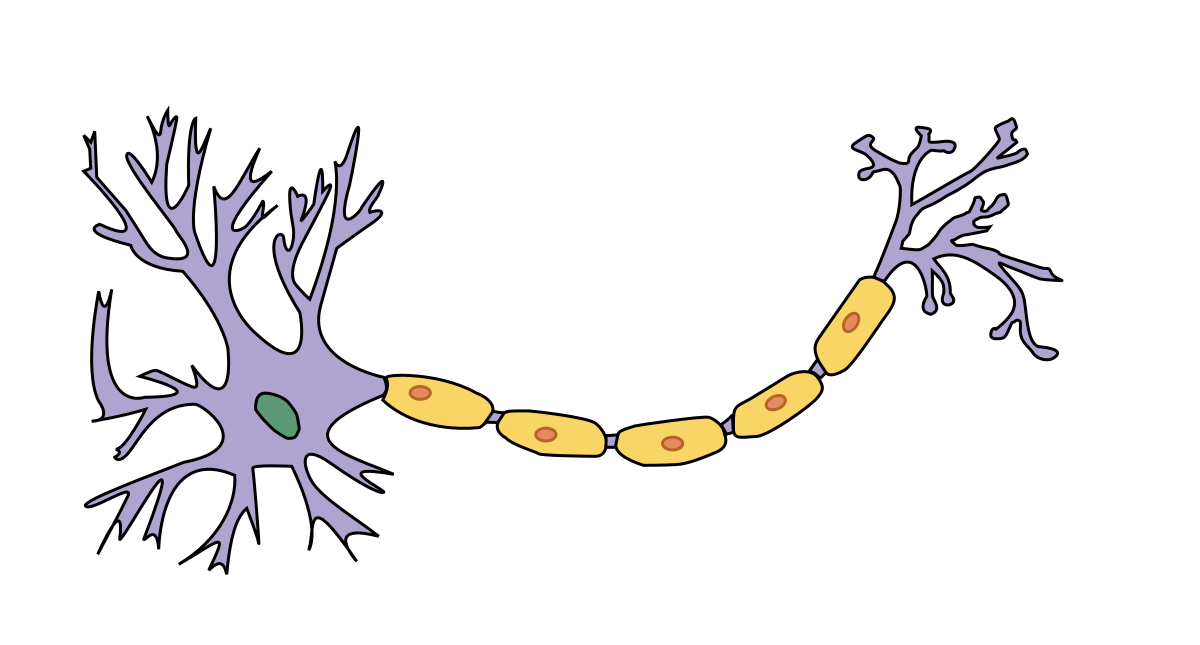
\includegraphics[width=0.8\textwidth]{neuron}
    \caption{Schematic representation of a neuron. \\
    {\small Image from \cite{WikimediaCommonsNeuron}}}
\end{figure}

One of the earliest models for neuronal activity is the \emph{McCulloch-Pitts model} \cite{McCulloch1943}, introduced in 1943. At the time, the understanding of how these cells work was limited, so the two researchers assumed that a neuron can have only one of two possible states (resting or firing). This led them to conclude that the activity of the whole brain could be modelled using propositional logic.

% TODO: finish talking about biological neurons

% TODO: talk about Hebb's rule for learning, Long-Term Potentation and Depression, more modern developments

\subsection{The Perceptron}

In 1957, while working at the Cornell Aeronautical Laboratory, the psychologist Frank Rosenblatt constructed what is widely considered to be the first learning machine to employ an artificial neural network \cite{Rosenblatt1957}.

% TODO: read the original paper (https://www.cs.cmu.edu/~./epxing/Class/10715/reading/McCulloch.and.Pitts.pdf) and cite it (https://link.springer.com/article/10.1007/BF02478259)

% TODO: talk about Rosenblatt's original perceptron algorithm (https://en.wikipedia.org/wiki/Perceptron)
% TODO: cite https://blogs.umass.edu/brain-wars/files/2016/03/rosenblatt-1957.pdf

Inspired by the simple McCulloch-Pitts model, Rosenblatt envisioned a neuron as performing a linear mapping on its inputs and then applying a threshold to determine if it should ``fire''.

\begin{definition}
The \emph{perceptron} is a binary classifier \(P \colon \reals^n \to \Set{0, 1}\) given by
\[
    P_{w, \, b} (x) = \begin{cases}
        1, \text{ if } w \cdot x + b \geq 0 \\
        0, \text{ otherwise}
    \end{cases}
\]
where \(w \in \reals^{1 \times n}\) and \(b \in \reals\) are trainable parameters, learned from the data.
\end{definition}

A neuron under the perceptron model would learn using the following algorithm:
\begin{enumerate}
    \item Choose a \emph{learning rate} \(\alpha > 0\) and initialize \(w\) and \(b\) to some (small) random values, or to zero.
    
    \item For each example \(\left(x, y\right)\) in the training data:
    \begin{itemize}
        \item Compute the current response of the neuron: \(\widehat{y} = P_{w, b} (x)\)

        \item Update the weights accordingly: \(w \xleftarrow{} w + \alpha (y - \widehat{y}) \cdot x\)
    \end{itemize}
\end{enumerate}

% TODO: discussion on a perceptron's mistake bounds: https://arxiv.org/pdf/1305.0208.pdf

Rosenblatt also considered networks with several layers of neurons, but at the time he could not find a working algorithm for training them.

% \subsection{Ivakhnenko's GMDH}

% In parallel with the developments in America, the Soviet-Ukrainian mathematician Alexey Ivakhnenko became interested in the theory of automatic control and developed the \emph{group method of data handling} (GMDH), which could accurately be described as the first instance of training a deep (neural) network.

% TODO: talk about Group Method of Data Handling https://en.wikipedia.org/wiki/Group_method_of_data_handling

% TODO: quote Ivachenko's paper, http://gmdh.net/articles/history/polynomial.pdf

\subsection{Deep Neural Networks}

\begin{definition}
A fully-connected \emph{layer} in a neural network is a  parameterized function
\begin{align*}
    f_{W, \, b} &\colon \reals^d \to \reals \\
    f_{W, \, b} (x) &= h\left(W x + b\right)
\end{align*}
where \(W \in \reals^d, b \in \reals\) are the \emph{layer weights} and \(h \colon \reals \to \reals\) is a non-linear \emph{activation function}.
\end{definition}

\begin{definition}
A feed-forward \emph{artificial neural network} is a parameterized function \(f_{\theta}\) obtained by composing several layers:
\[
    f_{\theta} (x) = f^{(n)}_{W_n, \, b_n} \left(\dots f^{(2)}_{W_2, \, b_2} (f^{(1)}_{W_1 \, b_1} (x))\right)
\]
\end{definition}

% \subsubsection{Backward propagation of errors}

The most commonly used algorithm for training neural networks with (multiple) hidden layers is the \emph{backward propagation of errors}. It was popularized by Rumelhart, Hinton and Williams in a paper from 1986 \cite{Rumelhart1986}, and versions of it have since been used ubiquitously.

% TODO: describe backprop algorithm, chain rule etc.

% TODO: talk about issues during training, instability, saddle points and so on

% \subsubsection{NNs as Universal Function Approximators}

% TODO: talk about the original version of the universal approximation theorem, and then some other variations
% https://en.wikipedia.org/wiki/Universal_approximation_theorem

\chapter{Auxiliary Models}

While not used to model the learning process \textit{per se}, this chapter presents a few mathematical theories which are very helpful in improving or understanding the learning algorithms described previously.

% \section{Physics-Informed Neural Networks}

% TODO: describe how imposing physical restrictions helps networks produce realistic solutions; maybe link to the philosophical "framing problem"

\section{Optimal Transport}

Transportation theory studies the problem of how to most efficiently move a mass of resources from point A to point B. The first mathematical analysis of the problem was given by Gaspard Monge in 1781 \cite{Monge1781}. A comprehensive, modern overview of the field is given in \cite{Villani2009}.

In the following, let \(\left(X, \mu\right)\) and \(\left(Y, \nu\right)\) be two probability spaces and let \(c \colon X \times Y \to \reals_{+}\) be a Borel-measurable \emph{cost function}.

\begin{definition}
A \emph{transport plan} is a measurable map \(T \colon X \to Y\) for which \(T_{*} \mu = \eta\), i.e.\ it \emph{preserves mass}.
\end{definition}

\begin{definition}
The \emph{total transporation cost} of a transport plan \(T\) is the value of the integral
\[
    C(T) = \int_{X} \, c\left(x, T(x)\right) \diff \mu(x)
\]
\end{definition}

\begin{definition}
An \emph{optimal transport plan} is a transport plan \(T\) which minimizes the \emph{total transportation cost}.
\end{definition}

In other words, an optimal transport plan satisfies
\[
    \arginf_{\substack{T \colon X \to Y \\ T_{*} \mu = \eta}} C(T)
\]

A priori, we have no reason to believe that a minimizer to the optimization problem exists. The Soviet mathematician Leonid Kantorovich gave a different formulation of the optimal transport problem, which made it much easier for him to prove the existence of at least one such map.

\begin{definition}
A \emph{coupling} is a probability measure \(\gamma\) on \(X \times Y\) whose marginal probability on \(X\) is \(\mu\) and on \(Y\) is \(\nu\). More precisely,
\begin{align*}
    \int_{Y} \gamma(x, y) \diff y &= \mu(x) \\
    \int_{X} \gamma(x, y) \diff x &= \nu(y)
\end{align*}
The set of all couplings is denoted by \(\Gamma(\mu, \nu)\).
\end{definition}

In Kantorovich's formulation, the optimal transport problem is restated as finding the coupling which minimizes the total cost:
\[
    \arginf_{\gamma \in \Gamma(\mu, \nu)} \int_{X \times Y} c(x, y) \diff \gamma(x, y)
\]
With this reinterpretation of the problem, it is now possible to prove the existence of a solution. See, for example, Theorem 4.1 from \cite{Villani2009}. It relies on Prokhorov's theorem \cite{Prokhorov1956}, a result from measure theory which characterizes precompact sets in the weak topology of measures. % TODO

\subsection{Wasserstein Distances}

In the statistics literature, one of the most popular uses of optimal transport theory is the definition of the \emph{Wasserstein distance} between two probability distributions.

\begin{definition}
The \emph{Wasserstein \(p\)-distance} is
\begin{align*}
    W_p (\mu, \nu) &= \left(\inf_{\gamma \in \Gamma(\mu, \nu)} \expectedvalue_\gamma \left[\norm{x - y}^p\right]\right)^{1/p} \\
    &= \left(\inf_{\gamma \in \Gamma(\mu, \nu)} \int \norm{x - y}^p \diff \probability_{\gamma} (x, y) \right)^{1/p}
\end{align*}
\end{definition}

The Wasserstein distances are a natural choice of metric in the space of probability distributions, with many useful properties \cite{Panaretos2019}, making them attractive for certain machine learning applications \cite{Arjovsky2017}. Unfortunately, the computational cost associated with them is quite prohibited. The situation changed in 2013 with the introduction of \emph{Sinkhorn distances} by Cuturi \cite{Cuturi2013}. This related family of distances is obtained by including an \emph{entropic regularization term} in the optimal transport problem formulation.

\begin{definition}
Let \(p\) be a discrete probability distribution over \(i \in \Set{ 1, 2, \dots, d }\). The information-theoretical \emph{entropy} of \(p\) is
\[
    h(p) = - \sum_{i = 1}^{d} p_i \log p_i
\]
\end{definition}

\begin{remark*}
In the discrete case, a transport plan (joint probability distribution) between two discrete probability distributions \(p\) and \(q\) can be represented by a matrix \(T\), where the \(i\)th row sums to \(p_i\) and the \(j\)th column sums to \(q_j\).
\end{remark*}

\begin{definition}
Let \(p\), \(q\) be two discrete probability distributions over \(\Set{ 1, 2, \dots, d }\) and \(T\) a transport plan between them. The \emph{entropy} of \(T\) is
\[
    h(T) = - \sum_{i, j = 1}^{d} T_{i, j} \log T_{i, j}
\]
\end{definition}

\begin{definition}
Let \(T\) and \(S\) be two transport plans. Their \emph{Kullback-Leibler divergence} is
\[
    \symrm{KL} \divergence{T}{S} = \sum_{i, j = 1}^{d} T_{i, \, j} \log \frac{T_{i, \, j}}{S_{i, \, j}}
\]
\end{definition}

Cuturi's idea was to define a convex set in the space of couplings. Let \(U(p, q)\) denote the space of all couplings between \(p\) and \(q\). Then
\[
    U_{\alpha} (p, q) = \Set{ T \in U(p, q) | \symrm{KL} \divergence{T}{p q^{T}} \leq \alpha}
\]

\begin{definition}
The \emph{Frobenius inner product} between two matrices \(A\) and \(B\) is
\[
    \innerproduct{A}{B} = \Tr\left(A^{T} B\right)
\]
\end{definition}

\begin{definition}
The \emph{Sinkhorn distance} between two discrete probabilty distributions \(p\) and \(q\) is
\[
    d_{M, \alpha} (p, q) = \inf_{T \in U_{\alpha} (p, q)} \innerproduct{T}{M}
\]
where \(M\) is a (pairwise) distance matrix.
\end{definition}

Cuturi proved that, as \(\alpha\) tends to \(+\infty\), \(d_{M, \alpha}\) tends to the optimal transport distance.

% \begin{definition}
% Let \(\mu_1, \dots, \mu_n\) be a set of probability distributions on the same space. The \emph{Wasserstein \(p\)-barycenter} is the probability distribution \(\beta\) which minimizes
% \[
%     \sum_{i = 1}^{n} W_p \left(\beta, \mu_i\right)
% \]
% \end{definition}


% TODO: discuss how Wasserstein barycenters can be computed quickly

% \section{Entropy-Regularized Optimal Transport}

% TODO: talk about entropy-regularized optimal transport,
% i.e. the addition of an entropy term to the Kantorovich formulation makes the corresponding minimization problem strongly convex

% Unbalanced Minibatch Optimal Transport, applications to Domain Adaptation: \url{http://proceedings.mlr.press/v139/fatras21a/fatras21a.pdf}

% Optimal Transport and Deep Learning : Learning from one another:
% \url{https://theses.hal.science/tel-03544757/document}

\section{Information Geometry}

Information geometry aims to study the parameter spaces of various families of probability distributions and the natural geometric structure they can be endowed with.

The first steps in discovering this connection were taken by C. Rao in 1945 \cite{Rao1945}. The Indian school of statistics was interested in finding the best way of defining a ``distance'' between various parameterized distributions. Rao observed that the Fisher information matrix (a concept we will define below) can be interpreted as a Riemannian metric. 

Consider for example the family of normal distributions \(\normal{\mu}{\sigma^2}\), where \(\mu \in \reals\) is the mean and \(\sigma^2 \in \left[0, +\infty\right)\) is the variance. The corresponding parameterised probability density function is given by
\[
    p \left(x; \mu, \sigma^2\right) = \frac{1}{\sqrt{2 \pi} \sigma} \cdot e^{- \frac{(x - \mu)^2}{2 \sigma^2}}
\]
Denote the parameters of this distribution by \(\theta = \left(\mu, \sigma^2\right)\). The set of all \(\theta\)s, \(\reals \times \left[0, +\infty\right)\), could be identified with the upper half-plane in \(\reals^2\). However, this is not the only way we could parameterize this family of distributions. What we are going to show is that, in a certain sense, the geometry of the underlying space is the same, no matter which coordinate system we choose.

Furthermore, information geometry also provides a better description for the \emph{distance} between two distributions within the same family. In the example above, as \(\sigma\) gets smaller, the normal distribution gets more tightly packed together, and the difference (in absolute value) between the means is much more pronounced.

\subsection{Maximum Likelihood Estimation}

Parameterized probability distributions arise naturally when doing statistical modelling \cite{Rossi2018}. The context of the problem is as follows: we are given a sequence of i.i.d.\ random variables \(X_1, \dots, X_n\) and we want to determine the distribution \(\Tilde{p}\) which they are sampled from. We use domain-specific knowledge to assert that the true probability distribution \(\Tilde{p}\) is contained within a parametric family of probability distributions \(p(\cdot; \theta)\), with \(\theta \in \reals^d\). We want to determine the value of \(\theta\) which gives us \(p(\cdot; \theta) = \Tilde{p}\) using only the observed values of the random variables.

\begin{definition}
The \emph{likelihood function} \(\symcal{L}\) is
\[
    \symcal{L} \left(\theta\right) = p\left(x; \theta\right)
\]
\end{definition}

In other words, we simply took the joint probability distribution \(p\left(x; \theta\right)\) and viewed it as a function of \(\theta\), not of \(x\).

When selecting a model by finding the maximum of the likelihood function, we are doing \emph{maximum likelihood estimation}. If the likelihood function is differentiable, one useful information we can obtain from it is the score.

\begin{definition}
The \emph{score} is the gradient of the logarithm of the likelihood function, i.e.\
\[
    s(\theta) = \nabla_{\theta} (\log \symcal{L}) (\theta)
\]
\end{definition}

Besides determining the values of \(\theta\) for which the maximum likelihood is reached, we would also want to understand if the maximum is stable or not. The Fisher information matrix was introduced just for that.

\begin{definition}
The \emph{Fisher information matrix} for a parameterized probability distribution \(p(x; \theta)\) is
\[
    \left[I\left(\theta\right)\right]_{i, j} = \expectedvalue_{\theta} \left[\left(\frac{\partial}{\partial \theta_i} \log p\left(X; \theta\right)\right) \left(\frac{\partial}{\partial \theta_j} \log p\left(X; \theta\right)\right)\right]
\]
\end{definition}

When the Fisher information matrix evaluated at a certain point \(\theta\) in the parameter space is ``big'', it means that (the absolute value of) the score is often high around that parameter.

\begin{definition}
A \emph{statistical manifold} is a differentiable manifold where the individual points correspond to probability distributions.
\end{definition}

It turns out that Fisher information matrix endows the corresponding statistical manifold with a \emph{Riemannian metric}. This observation forms the basis of information geometry \cite{Amari2016}.

\subsection{Natural Gradient}

In his paper from 1998 \cite{Amari1998}, Amari (one of the founders of information geometry) remarked that a neural network's parameter space could be viewed as a Riemannian manifold. Hence, to determine the direction of steepest descent, it wasn't enough to consider the gradient of the loss function with respect to the weights; it is necessary to also properly take into account the geometry of the underlying manifold. This gives rise to a family of optimization methods based on the concept of the \emph{natural gradient}.

% TODO: read this overview on the use of Natural Policy Gradient methods in Reinforcement Learning https://arxiv.org/pdf/2209.01820.pdf

% TODO: this https://arxiv.org/abs/1412.1193

\begin{definition}
Let \(L \colon M \to \reals\) be a differentiable function defined on a Riemannian manifold \(M^n\). The \emph{natural gradient} of \(L\) is given by
\[
    \Tilde{\nabla} L (w) = G^{-1} (w) \nabla L (w)
\]
where \(G^{-1} = \left(g^{i j}\right)\) is the inverse metric tensor and \(\nabla L\) is the usual (Euclidean) gradient, computed by viewing the manifold as embedded in \(\reals^n\).
\end{definition}

% gradient is given locally by
% \[
%     \nabla L (w) = \begin{pmatrix}
%         \frac{\partial L}{w_1} \\
%         \hdots \\
%         \frac{\partial L}{w_n}
%     \end{pmatrix}
% \]

\begin{theorem}[Amari]
The direction of steepest descent of \(L\) (i.e. the direction in which the function \(L\) decreases the most) is given by \(-\Tilde{\nabla} L (w)\).
\end{theorem}

% \begin{proof}
%     % TO DO
% \end{proof}

The natural gradient became very popular after it was adopted in the reinforcement learning domain as the \emph{natural policy gradient} \cite{Kakade2001}.

% \subsubsection{Trust Region Policy Optimization}

% Natural gradient methods become really popular once they started being applied to reinforcement learning.
\chapter{Conclusions}

While the ultimate goal of constructing an artificial general intelligence still seems to be way in the distance, machine learning has been advancing quickly towards solving more and more advanced problems, with no end in sight for the current wave of progress. However, the field has known setbacks and periods of little activity, and there is no guarantee such bottlenecks will not occur again.

Fortunately, nowadays we know a lot more about intelligence and the human brain than we did over 50 years ago. We have rigorous theoretical frameworks for the problem of learning, allowing us to understand the trade-offs involved in constructing machines capable of improving based on previous experience.

It is my hope that the results presented here showcase the importance of performing a thorough rigorous analysis of the problem at hand, before jumping to solving it and evaluating the empirical performance of the solution. The limit of how powerful the intelligent machines we construct isn't only computational power or the availability of large data sets, but also the intrinsic difficulty of the concepts we are trying to learn and the bounded capacity of our models.

% TODO: add an extra idea or two here


%% Appendices
\appendix

\chapter{Linear Algebra}

A very good introduction to linear algebra is the book by Axler \cite{Axler2014}. A great overview is the series of videos by Grant Sanderson \cite{3Blue1Brown_EssenceOfLinearAlgebra}.

\begin{definition}[Vector space]
A \emph{vector space} over \(\reals\) is a set \(V\) equipped with a binary operation \(+\) and a multiplication by elements from \(\reals\), such that the following hold:
\begin{itemize}
    \item Associativity: \(\left(v_1 + v_2\right) + v_3 = v_1 + \left(v_2 + v_3\right)\), for all \(v_1, v_2, v_3 \in V\);
    \item Commutativity: \(u + v = v + u\), for all \(u, v \in V\);
    \item Neutral element for vector addition: there exists a \(0 \in V\) such that \(0 + v = v + 0 = v\), for all \(v \in V\);
    \item Additive inverse: for every \(v \in V\) there exists a vector \(-v \in V\) such that \(v + (-v) = 0\);
    \item Neutral element for scalar multiplication: the identity of the field acts trivially: \(1 v = v\), for all \(v \in V\);
    \item Scalar multiplication commutes with field multiplication: \(a (bv) = (ab) v\), for all \(a, b \in \reals\) and \(v \in V\);
    \item Scalar multiplication distributes over vector addition: \(a \left(v_1 + v_2\right) = a v_1 + a v_2\), for all \(a \in \reals\) and \(v_1, v_2 \in V\);
    \item Scalar multiplication distributes over field addition: \((a + b) v = a v + b v\), for all \(a, b \in \reals\) and \(v \in V\).
\end{itemize}
\end{definition}

\begin{definition}[Vector subspace]
A \emph{vector subspace} is a subset \(W \subseteq V\) if \(W\) is a vector space in itself, with the operations restricted from \(V\).
\end{definition}

\begin{remark*}
The definition of a vector subspace amounts to checking that
\begin{itemize}
    \item \(w_1 + w_2 \in W\), for all \(w_1, w_2 \in W\);
    \item \(a w \in W\), for all \(a \in \reals\) and \(w \in W\).
\end{itemize}
\end{remark*}

\begin{definition}[Direct sum]
The \emph{direct sum} of two vector subspaces \(W_1, W_2 \subseteq V\) with \(W_1 \cap W_2 = \Set{ 0 }\) is the set
\[
    W_1 \oplus W_2 = \Set{ w_1 + w_2 | w_1 \in W_1, w_2 \in W_2 }
\]
\end{definition}

\begin{definition}[Convex set]
\label{def:convex_set}

A subset \(C\) of a vector space \(X\) is called \emph{convex} if, for any \(x, y \in C\) and \(r \in [0, 1]\), the point \(r x + (1 - r) y\) is also in \(C\).
\end{definition}

\begin{definition}[Linear map]
A \emph{linear map} between two vector spaces \(V\), \(W\) is a function \(f \colon V \to W\) for which
\[
    f(\lambda_1 v_1 + \lambda_2 v_2) = \lambda_1 \, f(v_1) + \lambda_2 \, f(v_2)
\]
for all \(\lambda_1, \lambda_2 \in \reals\) and all \(v_1, v_2 \in V\).
\end{definition}

\begin{definition}[Kernel of a linear map]
The \emph{kernel} of a linear map \(f \colon V \to W\) is the set
\[
    \ker f = \Set{ v \in V | f(v) = 0 }
\]
\end{definition}

\begin{definition}[Image of a linear map]
The \emph{image} of a linear map \(f \colon V \to W\) is the set
\[
    \ima f = \Set{ w \in W | w = f(v) \text{ for some } v \in V }
\]
\end{definition}

\begin{proposition}
The kernel and the image of a linear map are vector subspaces (of the domain and of the codomain respectively).
\end{proposition}
\begin{proof}
Let \(v_1, v_2 \in \ker f\). Since \(f(v_1) = f(v_2) = 0\), we have that \(f(v_1 + v_2) = f(v_1) + f(v_2) = 0 + 0 = 0\). Furthermore, for any \(a \in \reals\), we have that \(f(a v_1) = a f(v_1) = a \cdot 0 = 0\).

Let \(w_1, w_2 \in \ima f\). Take \(v_1, v_2 \in V\) such that \(f(v_1) = w_1\), \(f(v_2) = w_2\). Then \(w_1 + w_2 = f(v_1) + f(v_2) = f(v_1 + v_2)\), which shows that \(w_1 + w_2 \in \ima f\). Analogously, for any \(a \in \reals\), we have that \(a w_1 = a f(v_1) = f(a v_1)\), whence \(a w_1 \in \ima f\).
\end{proof}

\begin{definition}[Linear functional]
A \emph{linear functional} or \emph{linear form} on a vector space \(V\) is a linear map \(\varphi \colon V \to \reals\) (with \(\reals\) viewed as a one-dimensional vector space over itself).
\end{definition}

\chapter{Functional Analysis}

A good reference for functional analysis is the classic book \cite{ReedSimon1972}.

\begin{definition}[Topology]
A \emph{topology} on a set \(X\) is a collection of subsets \(\tau \subseteq \powerset{X}\) such that the following hold:
\begin{itemize}
    \item the empty set \(\emptyset\) and \(X\) itself are in \(\tau\);
    \item \(\tau\) is closed under arbitrary unions: for any index set \(I\) and any \(\left(U_i\right)_{i \in I}\) such that \(U_i \in \tau\) for any \(i \in I\), we have \(\bigcup_{i \in I} U_i \in \tau\);
    \item \(\tau\) is closed under finite intersections: for any \(U_1, \dots, U_n \in \tau\), we have \(\bigcap U_i \in \tau\).
\end{itemize}
\end{definition}

\begin{definition}[Topological space]
A \emph{topological space} is a set \(X\) together with a topology \(\tau\) on it.
\end{definition}

\begin{definition}[Neighborhood]
Given a topological space \(\left(X, \tau\right)\), a \emph{neighborhood} of the point \(x \in X\) is any set \(U \in \tau\) which contains \(x\).
\end{definition}

\begin{definition}[Continuity at a point]
A function \(f \colon \left(X, \tau_X\right) \to \left(Y, \tau_Y\right)\) between two topological spaces is called \emph{continuous} at some point \(x\) if, for any neighborhood \(V \in \tau_Y\) of \(f(x)\), there exists a neighborhood \(U \in \tau_X\) such that \(f(U) \subseteq V\).
\end{definition}

\begin{definition}[Continuous function]
A function between two topological spaces is called \emph{continuous} if it is continuous at all points.
\end{definition}

\begin{definition}
A \emph{topological vector space} is a vector space \(V\) endowed with a topology \(\tau\), such that the vector addition and scalar multiplication maps are continuous.
\end{definition}

\begin{definition}
A \emph{continuous linear operator} is a linear map between two topological vector spaces \(\left(V, \tau_V\right)\) and \(\left(W, \tau_W\right)\) which is also continuous.
\end{definition}

\begin{definition}[Metric space]
A \emph{metric space} is a set \(X\) equipped with a \emph{distance function} \(d \colon X \times X \to \reals\), satisfying the following three properties:
\begin{itemize}
    \item \(d(x, y) \geq 0\), with \(d(x, y) = 0\) if, and only if, \(x = y\);
    \item \(d(x, y) = d(y, x)\);
    \item \(d(x, z) \leq d(x, y) + d(y, z)\);
\end{itemize}
for any \(x, y, z \in X\).
\end{definition}

\begin{definition}[Sequence]
Let \(X\) be a set. A \emph{sequence} in \(X\) is a function \(f \colon \naturals \to X\). Most commonly, it will be written as \(\left(x_n\right)_{n \in \naturals}\).
\end{definition}

\begin{definition}[Cauchy sequence]
Let \((X, d)\) be a metric space. The sequence \(\left(x_n\right)_{n \in \naturals}\) is called \emph{Cauchy} if, for any \(\varepsilon > 0\), there exists an \(N_{\varepsilon} \in \naturals\) such that \(d\left(x_i, x_j\right) < \varepsilon\) for any \(i, \, j > N_{\varepsilon}\).
\end{definition}

\begin{definition}[Convergence]
Let \((X, d)\) be a metric space. The sequence \(\left(x_n\right)_{n \in \naturals}\) is \emph{convergent to a point \(x \in X\)} if, for any \(\varepsilon > 0\), there exists an \(N_{\varepsilon} \in \naturals\) such that \(d\left(x, x_i\right) < \varepsilon\) for any \(i > N\).
\end{definition}

\begin{definition}[Complete metric space]
The metric space \((X, d)\) is called \emph{complete} if every Cauchy sequence is also convergent.
\end{definition}

\begin{definition}[Normed vector space]
A \emph{normed vector space} is a vector space \(V\) over a field \(F\) (we can assume it to be either \(\reals\) or \(\complex\)), equipped with a function \(\norm{\cdot} \colon V \to F\) which satisfies the following properties:
\begin{itemize}
    \item \(\norm{x} \geq 0\), with equality iff \(x = 0\);
    \item \(\norm{\lambda x} = \abs{\lambda} \norm{x}\);
    \item \(\norm{x + y} \leq \norm{x} + \norm{y}\);
\end{itemize}
for any \(x, y \in V\) and \(\lambda \in F\).
\end{definition}

\begin{definition}[Inner product space]
An \emph{inner product space} is a vector space \(V\) over a field \(F\), equipped with a function \(\innerproduct{\cdot}{\cdot} \colon V \times V \to F\) which satisfies the following properties:
\begin{itemize}
    \item \(\innerproduct{x}{y} = \overline{\innerproduct{y}{x}}\);
    \item \(\innerproduct{a x + b y}{z} = a \innerproduct{x}{z} + b \innerproduct{y}{z}\);
    \item \(\innerproduct{x}{x} \geq 0\), with equality iff \(x = 0\);
\end{itemize}
for any \(x, y, z \in V\) and \(a, b \in F\).
\end{definition}

\begin{remark*}
Every inner product also induces a norm, by setting \(\norm{x} \coloneq \innerproduct{x}{x}\).
\end{remark*}

\begin{definition}[Orthogonal complement]
The \emph{orthogonal complement} of a vector subspace \(W\) in an inner product space \(V\) is the set
\[
    W^{\perp} = \Set{ v \in V | \innerproduct{v}{w} = 0, \forall w \in W }
\]
\end{definition}

\begin{definition}[Hilbert space]
A \emph{Hilbert space} is an inner product space which is also complete with respect to the distance induced by the product.
\end{definition}

\begin{theorem}[Hilbert projection]
For every \(x \in H\) and every non-empty closed, convex set \(C \subseteq H\) there exists an unique \(p \in C\) for which minimizes the quantity \(\norm{x - p}\) over \(C\). In other words, \(\norm{x - p} \leq \norm{x - c}\) for all \(c \in C\). The point \(p\) is called the \emph{orthogonal projection} of \(x\) onto \(C\).
\end{theorem}

\begin{corollary}
Let \(G\) be a closed vector subspace of \(H\). Then \(H\) can be decomposed as
\(H = G \oplus G^{\perp}\).
\end{corollary}

\begin{definition}[Continuous dual space]
The \emph{continuous dual space} of a Hilbert space \(H\) is the vector space \(H^{\dual}\) consisting of all continuous linear functionals on \(H\).
\end{definition}

\begin{theorem}[Riesz representation]
Let \(H\) be a Hilbert space. For every continuous linear functional \(\varphi \in H^{\dual}\), there exists a unique vector \(x \in H\) such that
\[
    \varphi(y) = \innerproduct{y}{x}
\]
for all \(y \in H\), and the norm of the functional and the vector are the same,
\[
    \norm{\varphi}_{H^{\dual}} = \norm{x}_{H}
\]
\end{theorem}

\begin{corollary}
The dual space \(H^{\dual}\) is itself a Hilbert space.
\end{corollary}

\chapter{Probability Theory}

While some initial approaches to artificial intelligence involved formal representations of knowledge and symbolic reasoning, nowadays the field is firmly grounded in probabilistic methods. These are used to account for the imprecision in the algorithms' predictions, to quantify the uncertainty in our assumptions and beliefs, and to model the noise present in real-world training data. This appendix aims to give the reader a basic understanding of the mathematical theory of probability.

% TODO: cite relevant works about the history of symbolic AI and modern probabilistic/Bayesian methods


\section{Measure Theory}

Mathematicians wrote informal treatises on games of chance and random patterns for several hundred years before the first rigorous, axiomatic theory of probability emerged. The breakthrough which enabled this formalisation was Henri Lebesgue's abstract theory of integration, itself grounded in Camille Jordan's and Émile Borel's exploration of the concept of \emph{measure}.

% TODO: add citations to Lebesgue's and Borel's work
% https://en.wikipedia.org/wiki/Henri_Lebesgue
% https://en.wikipedia.org/wiki/%C3%89mile_Borel

A thorough introduction to measure theory is Terrence Tao's book \cite{Tao2011}, which we have used as reference material for this section. Another wonderful overview is given in J. P. Grossman's series of YouTube videos on this topic \cite{BSoM_MeasureTheory}

In order to properly define the concept of a measure, we will first need to specify the objects which we will be able to quantify. We will work with certain families of sets.
 
\begin{definition}[\(\sigma\)-algebra]
A \emph{\(\sigma\)-algebra} \(\symcal{F}\) on the set \(X\) is a collection of subsets of \(X\), such that the following conditions hold:
\begin{itemize}
    \item \(X\) itself is an element of \(\symcal{F}\);
    \item \(\symcal{F}\) is closed under taking complements, i.e.\ if \(E \in \symcal{F}\), then \(X \setminus E \in \symcal{F}\);
    \item \(\symcal{F}\) is closed under countable intersections, i.e.\ if \(E_1, E_2, \hdots \in \symcal{F}\), then
    \[
        \bigcap_{i \in \naturals^*} E_i \in \symcal{F}
    \]
\end{itemize}
\end{definition}

\begin{definition}
The \(\sigma\)-algebra \emph{generated} by a subset \(A \subseteq \powerset{X}\) is the smallest \(\sigma\)-algebra containing all the sets from \(A\). It is denoted by \(\sigma(A)\).
\end{definition}

\begin{definition}[Measurable space]
A \emph{measurable space} is a pair \(\left(X, \symcal{F}\right)\), where \(\symcal{F}\) is a \(\sigma\)-algebra on \(X\). An element \(E \in \symcal{F}\) is called a \emph{measurable set}.
\end{definition}

In the following, we will use the term \emph{space} interchangeably with \emph{measurable space}, when no ambiguity can arise.

\begin{definition}
Given two measurable spaces \(\left(X, \symcal{F}\right)\) and \(\left(Y, \symcal{G}\right)\), the \emph{product \(\sigma\)-algebra} on \(X \times Y\) is defined as
\[
    \symcal{F} \otimes \symcal{G} = \sigma\left(\Set{ (U, V) | U \in \symcal{F}, V \in \symcal{G} }\right)
\]
\end{definition}

\begin{definition}[Measure]
A \emph{measure} on the space \(\left(X, \symcal{F}\right)\) is a function \(\mu \colon \symcal{F} \to [0, +\infty]\), satisfying the following two properties:
\begin{itemize}
    \item Measure of the empty set is zero: \(\mu\left(\emptyset\right) = 0\);
    \item It is \(\sigma\)-additive: if \(E_1, E_2, \dots \in \symcal{F}\) is a countable sequence of disjoint sets, then
    \[
        \mu\left(\bigcup_{k = 1}^{\infty} E_{k}\right) = \sum_{k = 1}^{\infty} \mu\left(E_k\right)
    \]
\end{itemize}
\end{definition}

\begin{definition}[Measure space]
A \emph{measure space} is a triplet \(\left(X, \symcal{F}, \mu\right)\) where \(\left(X, \symcal{F}\right)\) is a measurable space and \(\mu\) is a measure on it.
\end{definition}

\begin{definition}[Complete measure]
\label{def:complete_measure}

A measure on \(\left(X, \symcal{F}\right)\) is called \emph{complete} if, for any \(E \in \symcal{F}\) with \(\mu(E) = 0\) and any \(F \subset E\) we have \(\mu(F) = 0\).
\end{definition}

\begin{definition}[Measurable function]
A function \(f \colon \left(X, \symcal{F}\right) \to \left(Y, \symcal{B}\right)\) between two measurable spaces is called \emph{measurable} if \(f^{-1} (B) \in \symcal{F}\) for every \(B \in \symcal{B}\).
\end{definition}

\begin{proposition}
The \emph{composition} \(g \circ f\) of two measurable functions \(f \colon \left(X, \symcal{F}\right) \to \left(Y, \symcal{B}\right)\) and \(g \colon \left(Y, \symcal{B}\right) \to \left(Z, \symcal{C}\right)\) is itself a measurable function.
\end{proposition}
\begin{proof}
For any \(G \in \symcal{C}\), we have
\[
    \left(g \circ f\right)^{-1} (G) = \left(f^{-1} \circ g^{-1}\right) (G) = f^{-1} \left(g^{-1} (G)\right)
\]
Using the fact that \(g\) is measurable, we deduce that \(g^{-1} (G) \in \symcal{B}\), and now because \(f\) is measurable, we obtain \(f^{-1} \left(g^{-1} (G)\right) \in \symcal{F}\).
\end{proof}

\begin{definition}[Push-forward measure]
The \emph{push-foward} of a measure \(\mu\) (on \(X\)) through a measurable function \(f \colon \left(X, \symcal{F}\right) \to \left(Y, \symcal{B}\right)\) is the measure \(\eta\) (on \(Y\)), defined by
\[
    \eta(F) = \left(f_{*} \mu\right) (F) = \mu \left(f^{-1} (F)\right)
\]
for any \(F \in \symcal{B}\).
\end{definition}

\section{Theory of Probability}

One of the first modern works to provide a rigorous foundation for probability theory using measure theory is Kolmogorov's book from 1933 \cite{Kolmogorov1933}.

\subsection*{Probability Spaces}

\begin{definition}[Probability measure]
A \emph{probability measure} on a set \(\Omega\) is a measure \(\probability\) on \(\Omega\) for which \(\probability(\Omega) = 1\).
\end{definition}

\begin{definition}[Probability space]
A \emph{probability space} is a measurable space \(\left(\Omega, \symcal{F}, \probability\right)\) for which \(\probability\) is a probability measure.
\end{definition}

\begin{remark*}
The measurable sets of \(\Omega\) are more commonly known as \emph{events}.
\end{remark*}

\begin{definition}[Complete probability space]
A probability space \(\left(\Omega, \symcal{F}, \probability\right)\) is called \(\emph{complete}\) if the probability measure \(\probability\) is complete (see definition \ref{def:complete_measure}).
\end{definition}

\begin{definition}[Conditional probability]
Let \(A, B \in \Omega\) be two events with \(\probability(B) \neq 0\). The \emph{conditional probability of \(A\) given \(B\)} is
\[
    \probability\given{A}{B} = \frac{\probability(A \cap B)}{\probability(B)}
\]
\end{definition}

\begin{theorem}[Bayes]
Let \(A, B \in \Omega\) be two events with \(\probability(B) \neq 0\). The following equality holds:
\[
    \probability\given{A}{B} = \frac{\probability\given{B}{A} \probability(A)}{\probability(B)}
\]
\end{theorem}
\begin{proof}
From the definition of conditional probability for \(\probability\given{A}{B}\), we get that
\[
    \probability(A \cap B) = \probability\given{A}{B} \probability(B)
\]
Doing the same for \(\probability\given{B}{A}\), we obtain
\[
    \probability(B \cap A) = \probability\given{B}{A} \probability(A)
\]
Since \(A \cap B = B \cap A\), we can connect the two equalities above to obtain
\[
    \probability\given{A}{B} \probability(B) = \probability\given{B}{A} \probability(A)
\]
Dividing by \(\probability(B)\) on both sides (we've assumed in the hypothesis that it is not zero) gives us the desired conclusion.
\end{proof}

\subsection*{Random Variables}

\begin{definition}[Random variable]
A \emph{random variable} \(X\) is a measurable function from a probability space \(\left(\Omega, \symcal{A}, \probability\right)\) to some measurable space \(\left(Y, \symcal{B}\right)\).
\end{definition}

\begin{remark*}
Most commonly we will consider random variables taking values in \(\reals\), on which we impose a measure space structure with the \emph{Borel \(\sigma\)-algebra} \(\borelsets{\reals}\) (the \(\sigma\)-algebra generated by all open sets).
\end{remark*}

\begin{definition}[Distribution of a random variable]
The \emph{distribution} of a random variable \(X \colon \Omega \to \reals\) is the push-forward measure \(\probability_X\) given by
\[
    \probability_X \left(B\right) = \probability\left(X^{-1} \left(B\right)\right)
\]
for all \(B \in \borelsets{\reals}\).
\end{definition}

\begin{definition}[Probability density function]
The \emph{probability density function} of \(X\) is a measurable function \(f_X \colon \reals \to \reals^{+}\) with the property that
\[
    \probability_X (B) = \int_{B} f_X (x) \diff x
\]
for any \(B \in \borelsets{\reals}\).
\end{definition}

\begin{remark*}
The density function of a random variable is unique up to sets of Lebesgue measure zero. Its existence is implied by the \emph{Radon-Nikodym theorem}.
\end{remark*}

\begin{definition}[Cumulative distribution function]
The \emph{cumulative distribution function} of a random variable \(X\) is
\begin{align*}
    F_X (x) &= \probability\left(X \leq x\right)
    = \probability_X \left((-\infty, x]\right) \\
    &= \probability\left(X^{-1} \left((-\infty, x]\right)\right)
    = \probability\left(\Set{ \omega \in \Omega | X(\omega) \leq x }\right)
\end{align*}
\end{definition}

\subsection*{Measurable Cross-Sections}

In the following discussion, let \(\left(\Omega, \symcal{F}, \probability\right)\) be a probability space and \(\left(T, d\right)\) a metric space, viewed as a measurable space endowed with the Borel \(\sigma\)-algebra \(\borelsets{T}\).

The original results in this section rely on the notion of \emph{analytic sets} associated with a \(\sigma\)-algebra. For simplicity, we will instead assume that \(\Omega \times T\) is a complete probability space (in this case, the measurable sets coincide with the ``analytic sets''). The interested reader can consult \cite{DellacherieMeyer1978} for the complete details. The only result we will require from there is the following:

\begin{theorem}[Measurable cross-section]
\label{thm:measurable_cross_section}

Let \(\left(\Omega \times T, \symcal{F} \otimes \borelsets{T}, \probability\right)\) be a complete probability space and \(A \in \symcal{F} \otimes \borelsets{T}\). Let \(\overline{T} = T \sqcup \Set{ \infty }\) and denote by \(\pi_{\Omega} \colon \Omega \times T \to \Omega\) the projection onto the first component. There exists a measurable map \(s \colon \Omega \to \overline{T}\), called a \emph{cross-section}, for which
\begin{itemize}
    \item \(s(\omega) \neq \infty\) implies that \(\left(\omega, s(\omega)\right) \in A\);
    \item \(\probability_{\pi_{\Omega}}\left(s(\omega) \neq \infty\right) = 1\).
\end{itemize}
\end{theorem}

The following theorem and its proof are based on \cite[p.~197]{Pollard1984}.

\begin{theorem}
\label{thm:pollard_supremum_of_stochastic_process}

Let \(\Set{ X_t }\) be a family of random variables indexed by \(t \in T\), such that \(X \colon \Omega \times T \to \reals\) is measurable and \(X_t = X(\cdot, t)\). Then there exists a random variable \(\tau \colon \Omega \to T\) such that
\[
    \probability\given{\abs{X_\tau} > \varepsilon}{\sup_{t \in T} \, \abs{X_t} > \varepsilon} = 1
\]
In other words, we have \(\abs{X_\tau} > \varepsilon\) almost surely whenever \(\sup_{t \in T} \abs{X_t} > \varepsilon\).
\end{theorem}
\begin{proof}
Let \(\Set{ \varepsilon_i }_{i \in \naturals}\) be a strictly decreasing sequence of (extended) real numbers, with \(\varepsilon_0 = \infty\). Define
\begin{align*}
    A_i &= \Set{ \omega \in \Omega | \varepsilon_{i + 1} < \sup_{t \in T} \, \abs{X(\omega, t)} \leq \varepsilon_i } \\
    B_i &= \Set{ (\omega, t) \in \Omega \times T | \varepsilon_{i + 1} < \abs{X(\omega, t)} \leq \varepsilon_i }
\end{align*}
The sets \(A_i\) and \(B_i\) are measurable, since
\begin{align*}
    A_i &= \left(\sup_{t \in T} \abs{X_t}\right)^{-1} \left(\left(\varepsilon_{i + 1}, \varepsilon_i\right]\right) \in \symcal{F} \\
    B_i &= \left(\abs{X}\right)^{-1} \left(\left(\varepsilon_{i + 1}, \varepsilon_{i}\right]\right) \in \symcal{F} \otimes \borelsets{T}
\end{align*}
(see \cite{AdamsNobel2010} for a discussion on the measurability of supremums of random variables)

Applying the previous theorem \ref{thm:measurable_cross_section}, we obtain a cross-section \(s_i \colon \Omega \to \overline{T}\) for each \(B_i\). Fix a \(t_0 \in T\). Define \(\tau \colon \Omega \to T\) as follows:
\[
    \tau(\omega) = \begin{cases}
        \tau_i (\omega) \text{ if } \omega \in A_i \text{ and } \tau_i (\omega) \neq \infty \\
        t_0 \text{ otherwise }
    \end{cases}
\]
For almost all \(\omega \in \Omega\), if \(\sup_{t \in T} \abs{X(\omega, t)} > \varepsilon\), then by definition we have \(\omega \in A_i\) for some \(i\) (say \(\varepsilon = \varepsilon_{i + 1}\)). By the properties of the cross-section, this means that \(\left(\omega, \tau(\omega)\right) \in B_i\), whence
\[
    \varepsilon = \varepsilon_{i + 1} < \abs{X(\omega, \tau(\omega))} \leq \varepsilon_i
\]
or in other words
\[
    \abs{X_\tau (\omega)} > \varepsilon
\]
\end{proof}

\subsection*{Expected Value}

\begin{definition}[Expected value]
The \emph{expected value} of the random variable \(X\) is the value of the integral
\[
    \expectedvalue\left[X\right] = \int_{-\infty}^{+\infty} x \diff \probability_X (x) = \int_{-\infty}^{+\infty} x \, f_X (x) \diff x
\]
\end{definition}

\begin{remark*}
The integral above is technically a Lebesgue integral, but for our purposes, interpreting it as a Riemann integral on \(\reals\) will suffice.
\end{remark*}

\begin{definition}
Let \(X \colon \Omega \to \reals\) be a random variable and \(g \colon \reals \to \reals\) a measurable function. The \emph{composition of \(g\) and \(X\)}, denoted by \(g(X)\), is the random variable \(g \circ X\).
\end{definition}

\begin{remark*}
By the properties of the Lebesgue integral, the expected value of the composite random variable is given by
\[
    \expectedvalue\left[g(X)\right] = \int_{-\infty}^{+\infty} g(x) \diff \probability_X (x) = \int_{-\infty}^{+\infty} g(x) \, f_{X} (x) \diff x
\]
\end{remark*}

\begin{proposition}[Properties of expected value]
For any \(X, Y\) random variables and \(a \in \reals\), the following hold:
\begin{enumerate}
    \item \(\expectedvalue[X + a] = \expectedvalue[X] + a\)
    \item \(\expectedvalue[a X] = a \expectedvalue[X]\)
    \item \(\expectedvalue[X + Y] = \expectedvalue[X] + \expectedvalue[Y]\)
\end{enumerate}
\end{proposition}
\begin{proof}
The properties follow from the definition of the expected value and the well-known properties of the integral.
\begin{enumerate}
    \item We apply a previous remark for the composition of \(X\) with the measurable function \(g(x) = x + a\).
    \begin{align*}
        \expectedvalue[X + a] &= \int_{-\infty}^{+\infty} (x + a) \, f_X (x) \diff x
        = \int_{-\infty}^{+\infty} x \, f_X (x) \diff x + \int_{-\infty}^{+\infty} a \, f_X (x) \diff x \\[0.5em]
        &= \expectedvalue[X] + a \int_{-\infty}^{+\infty} f_X (x) \diff x
        = \expectedvalue[X] + a
    \end{align*}

    \item We now compose \(X\) with the function \(g(x) = ax\).
    \[
        \expectedvalue[a X] = \int_{-\infty}^{+\infty} a \, x \, f_X (x) \diff x = a \int_{-\infty}^{+\infty} x \, f_X (x) \diff x = a \expectedvalue[X]
    \]

    \item We use the linearity of the integral.
    \begin{align*}
        \expectedvalue[X + Y] &= \int_{-\infty}^{+\infty} x \left(f_X (x) + f_Y (x)\right) \diff x \\
        &= \int_{-\infty}^{+\infty} x \, f_X (x) \diff x + \int_{-\infty}^{+\infty} x \, f_Y (x) \diff x \\
        &= \expectedvalue[X] + \expectedvalue[Y]
    \end{align*}
\end{enumerate}
\end{proof}

\subsection*{Variance and Covariance}

\begin{definition}[Variance]
The \emph{variance} of the random variable \(X\) is given by
\[
    \variance(X) = \expectedvalue\left[\left(X - \expectedvalue\left[X\right]\right)^2\right]
\]
\end{definition}

\begin{remark*}
A short computation will provide us with an alternative and often used formula for the variance:
\begin{align*}
    \variance(X) &= \expectedvalue\left[\left(X - \expectedvalue\left[X\right]\right)^2\right] = \expectedvalue\left[X^2 - 2 \cdot \expectedvalue\left[X\right] \cdot X + \left(\expectedvalue[X]\right)^2\right] \\
    &= \expectedvalue\left[X^2\right] - 2 \cdot \expectedvalue\left[X\right] \cdot \expectedvalue\left[X\right] + \left(\expectedvalue\left[X\right]\right)^2 \\
    &= \expectedvalue\left[X^2\right] - 2 \cdot \left(\expectedvalue\left[X\right]\right)^2 + \left(\expectedvalue\left[X\right]\right)^2 \\
    &= \expectedvalue\left[X^2\right] - \left(\expectedvalue\left[X\right]\right)^2
\end{align*}
\end{remark*}

\begin{definition}[Standard deviation]
The \emph{standard deviation} of a random variable \(X\) is given by
\[
    \sigma_X = \sqrt{\variance{X}}
\]
\end{definition}

\begin{definition}[Covariance]
The \emph{covariance} of two random variables is given by
\[
    \covariance(X, Y) = \expectedvalue\left[\left(X - \expectedvalue[X]\right) \left(Y - \expectedvalue(Y)\right)\right]
\]
\end{definition}

\begin{remark*}
We have that \(\covariance(X, X) = \variance(X)\).
\end{remark*}

\begin{proposition}[Properties of variance]
For any \(X, Y\) random variables and \(a \in \reals\), the following hold:
\begin{enumerate}
    \item \(\variance(X + a) = \variance(X)\)
    \item \(\variance(a X) = a^2 \variance(X)\)
    \item \(\variance(X + Y) = \variance(X) + \variance(Y) + 2 \covariance(X, Y)\)
\end{enumerate}
\end{proposition}
\begin{proof}
~
\begin{enumerate}
    \item This property follows from the definition of variance by simplifying the \(a\)s that appear:
    \begin{align*}
        \variance(X + a) &= \expectedvalue\left[\left(\left(X + a\right) - \expectedvalue\left[X + a\right]\right)^2\right] \\
        &= \expectedvalue\left[\left(X + \cancel{a} - \expectedvalue[X] + \cancel{a}\right)^2\right] \\
        &= \expectedvalue\left[\left(X - \expectedvalue[X]\right)^2\right] = \variance(X)
    \end{align*}

    \item This property follows by using the definition of variance and pulling out the common \(a\) factor:
    \begin{align*}
        \variance(a X) &= \expectedvalue\left[\left(a X - \expectedvalue\left[a X\right]\right)^2\right] \\
        &= \expectedvalue\left[\left(a \left(X - \expectedvalue\left[X\right]\right)\right)^2\right] \\
        &= \expectedvalue\left[a^2 \left(X - \expectedvalue\left[X\right]\right)^2\right] \\
        &= a^2 \expectedvalue\left[\left(X - \expectedvalue\left[X\right]\right)^2\right] = a^2 \variance(X)
    \end{align*}

    \item For this property, we use the definition of variance, apply the linearity of the expected value and regroup conveniently:
    \begin{align*}
        \variance(X + Y) &= \expectedvalue\left[\left(\left(X + Y\right) - \expectedvalue\left[\left(X + Y\right)\right]\right)^2\right] \\
        &= \expectedvalue\left[\left(X + Y - \expectedvalue\left[X\right] - \expectedvalue\left[Y\right]\right)^2\right] \\
        &= \expectedvalue\left[\left((X - \expectedvalue[X]) + (Y - \expectedvalue[Y])\right)^2\right] \\
        &= \expectedvalue\left[(X - \expectedvalue[X])^2 + (Y - \expectedvalue[Y])^2 + 2 (X - \expectedvalue[X]) (Y - \expectedvalue[Y])\right] \\
        &= \expectedvalue\left[(X - \expectedvalue[X])^2\right] + \expectedvalue\left[(Y - \expectedvalue[Y])^2\right] + \\
        &\qquad\quad + 2 \expectedvalue\left[(X - \expectedvalue[X]) (Y - \expectedvalue[Y])\right] \\
        &= \variance(X) + \variance(Y) + 2 \covariance(X, Y)
    \end{align*}
\end{enumerate}
\end{proof}

\subsection*{Markov's and Chebyshev's Inequalities}

\begin{theorem}[Markov's Inequality]
Let \(X \colon \Omega \to \reals^+\) be a non-negative random variable and let \(a > 0\). Then
\[
    \probability\left(X \geq a\right) \leq \frac{\expectedvalue\left[X\right]}{a}
\]
\end{theorem}
\begin{proof}
By definition, the expected value of \(X\) is
\[
    \expectedvalue\left[X\right] = \int_{-\infty}^{+\infty} x \diff \probability_X (x) = \int_{-\infty}^{+\infty} x \, f_X (x) \diff x
\]
Since our random variable is assumed to be non-negative, we can rewrite this as
\[
    \expectedvalue\left[X\right] = \int_{0}^{+\infty} x \, f_X (x) \diff x = \int_{0}^{a} x \, f_X (x) \diff x + \int_{a}^{+\infty} x \, f_X (x) \diff x
\]
Because the product \(x \, f_X (x)\) is positive and certainly finite from \(0\) to \(a\), we can provide a lower bound for the expected value of \(X\):
\[
    \expectedvalue\left[X\right] \geq \int_{a}^{+\infty} x \, f_X (x) \diff x
\]
Furthermore, we can lower bound \(x \, f_X (x)\) by \(a \, f_X (x)\), giving us
\[
    \expectedvalue\left[X\right] \geq \int_{a}^{+\infty} a \, f_X (x) \diff x = a \int_{a}^{+\infty} f_X (x) \diff x = a \cdot \probability\left(X \geq a\right)
\]
whence, dividing by \(a\) on both sides, we obtain
\[
    \frac{\expectedvalue\left[X\right]}{a} \geq \probability\left(X \geq a \right)
\]
as claimed.
\end{proof}

\begin{theorem}[Chebyshev's Inequality]
\label{thm:chebyshev_inequality}
Let \(X\) be a random variable with finite expected value \(\mu\) and finite standard deviation \(\sigma\). For any \(t > 0\), we have
\[
    \probability\left(\abs{X - \mu} \geq t \sigma\right) \leq \frac{1}{t^2}
\]
\end{theorem}
\begin{proof}
Squaring both sides of the inner inequality, we get
\[
    \probability\left(\abs{X - \mu} \geq t \sigma\right) = \probability\left(\left(X - \mu\right)^2 \geq t^2 \sigma^2\right)
\]
We can now apply Markov's inequality to the random variable \(\left(X - \mu\right)^2\), taking \(a = t^2 \sigma^2\), which gives us
\[
    \probability\left(\left(X - \mu\right)^2 \geq t^2 \sigma^2\right) \leq \frac{\expectedvalue\left[\left(X - \mu\right)^2\right]}{t^2 \sigma^2} = \frac{\bcancel{\variance(X)}}{t^2 \cdot \bcancel{\variance(X)}} = \frac{1}{t^2}
\]
\end{proof}

\begin{definition}
\label{def:identically_distributed}

A family \(\Set{ X_i }_{i \in I}\) of random variables is said to be \emph{identically distributed} if
\[
    F_{X_i} (x) = F_{X_j} (x)
\]
for all \(x \in \reals\), \(i, j \in I\).
\end{definition}

\begin{definition}
\label{def:independence}

A family \(\Set{ X_i }_{i \in I}\) of random variables is said to be \emph{independent} if
\[
    F_{X_{i_1}, \dots, X_{i_n}} (x) = F_{X_{i_1}} (x) \cdot \dots \cdot F_{X_{i_n}} (x) 
\]
for all \(x \in \reals\), \(n \in \naturals\) and \(i_1, \dots, i_n \in I\).
\end{definition}

\begin{definition}
A family \(\Set{ X_i }\) of random variables is said to be \emph{independent and identically distributed} (\emph{i.i.d.}) if it respects the conditions stated in definitions \ref{def:identically_distributed} and \ref{def:independence}.
\end{definition}

\begin{definition}[Sample average]
The \emph{sample average} of a sequence \(X_1, \dots, X_n\) of random variables is
\[
    \overline{X}_n = \frac{1}{n} \sum_{i = 1}^{n} X_i
\]
\end{definition}

\begin{theorem}[Weak law of large numbers]
\label{thm:weak_law_of_large_numbers}

Let \(X_1, \dots, X_n\) be a sequence of i.i.d.\ random variables with expected value \(\mu\). Then for any real number \(\varepsilon > 0\), we have
\[
    \lim_{n \to \infty} \probability\left(\abs{\overline{X}_n - \mu} \geq \varepsilon\right) = 0
\]
\end{theorem}
\begin{proof}
We intend to apply Chebyshev's inequality. Clearly, the expected value of the sample average is the same as the mean of any individual variable: \(\expectedvalue\left[\overline{X}_n\right] = \mu\).

Since the variables are independent, their covariance is \(0\). This allows us to compute the variance of the sample mean as
\[
    \variance\left(\overline{X}_n\right) = \variance\left(\frac{1}{n} \sum_{i = 1}^{n} X_i\right) = \frac{1}{n^2} \sum_{i = 1}^{n} \variance\left(X_i\right) = \frac{1}{n^2} \cdot n \cdot \sigma^2 = \frac{\sigma^2}{n}
\]
Hence, the standard deviation is \(\frac{\sigma}{\sqrt{n}}\).

Chebyshev's inequality now tells us that
\[
    \probability\left(\abs{\overline{X}_n - \mu} \geq t \frac{\sigma}{\sqrt{n}}\right) \leq \frac{1}{t^2}
\]
for any \(t > 0\). Letting \(\varepsilon \coloneq t \sigma / \sqrt{n}\), we have \(t^2 = \varepsilon^2 n / \sigma^2\). Substituting, we obtain
\[
    \probability\left(\abs{\overline{X}_n - \mu} \geq \varepsilon\right) \leq \frac{\sigma^2}{\varepsilon^2 n}
\]
When \(n\) tends to infinity, the right-hand side of the inequality tends to \(0\), as claimed.
\end{proof}

\subsection*{Hoeffding's Inequality}

\begin{definition}
The \emph{\(k\)-th moment} of a random variable \(X\) is
\[
    m_k (X) = \expectedvalue\left[X^k\right]
\]
\end{definition}

\begin{definition}[Moment-generating function]
The \emph{moment-generating function} of a random variable \(X\) is
\[
    M_X (t) = \expectedvalue\left[e^{t X}\right]
\]
\end{definition}

\begin{remark*}
The series expansion of \(e^{t X}\) is
\[
    e^{t X} = 1 + \frac{t \, X}{1!} + \frac{t^2 \, X^2}{2!} + \dots + \frac{t^k \, X^k}{k!} + \dots
\]
whence the expected value is
\begin{align*}
    \expectedvalue\left[e^{t X}\right] &= 1 + \frac{t \, \expectedvalue\left[X\right]}{1!} + \frac{t^2 \, \expectedvalue\left[X^2\right]}{2!} + \dots + \frac{t^k \, \expectedvalue\left[X^k\right]}{k!} + \dots \\
    &= 1 + \frac{t \, m_1 (X)}{1!} + \frac{t^2 \, m_2 (X)}{2!} + \dots + \frac{t^k \, m_k (X)}{k!} + \dots
\end{align*}
This justifies the name ``moment-generating function''.
\end{remark*}

\begin{lemma*}[Hoeffding's lemma]
Let \(X\) be a random variable which is bounded almost-surely, i.e.\ there exist \(a, b \in \reals\) such that \(\probability\left(a \leq X \leq b\right) = 1\). Then, for any \(\lambda > 0\), we have
\[
    \expectedvalue\left[e^{\lambda X}\right] \leq e^{\lambda \expectedvalue[X] + \frac{\lambda^2 (b - a)^2}{8}}
\]
\end{lemma*}
\begin{proof}
Note that
\[
    \expectedvalue\left[e^{\lambda \left(X - \expectedvalue[X]\right)}\right] = \expectedvalue\left[e^{\lambda X} e^{-\lambda \expectedvalue[X]}\right] = \expectedvalue\left[e^{\lambda X}\right] \cdot e^{-\lambda \expectedvalue[X]}
\]
So we can assume that \(X\) has mean \(0\) and prove only that
\[
    \expectedvalue\left[e^{\lambda X}\right] \leq e^{\frac{\lambda^2 (b - a)^2}{8}}
\]

Since \(f(x) = e^{\lambda x}\) is a convex function, we can apply Jensen's inequality \cite{Jensen1906} on the interval \([a, b]\) to obtain
\[
    e^{\lambda x} \leq \frac{b - x}{b - a} e^{\lambda a} + \frac{x - a}{b - a} e^{\lambda b}
\]
for all \(x \in [a, b]\). By the linearity of the expected value, we get
\begin{align*}
    \expectedvalue\left[e^{\lambda X}\right] &\leq \expectedvalue\left[\frac{b - X}{b - a} e^{\lambda a} + \frac{X - a}{b - a} e^{\lambda b}\right]
    = \frac{b - \expectedvalue[X]}{b - a} e^{\lambda a} + \frac{\expectedvalue[X] - a}{b - a} e^{\lambda b} \\[0.5em]
    &= \frac{b}{b - a} e^{\lambda a} + \frac{-a}{b - a} e^{\lambda b}
    = e^{\lambda a} \left(\frac{b}{b - a} + \frac{- a}{b - a} e^{\lambda b - \lambda a}\right) \\[0.5em]
    &= e^{\lambda a} e^{\ln \left(\frac{b}{b - a} + \frac{- a}{b - a} e^{\lambda (b - a)}\right)}
    = e^{\lambda a + \ln \left(\frac{b - a e^{\lambda (b - a)}}{b - a}\right)} \\[0.5em]
    &= e^{\frac{\lambda (b - a) a}{b - a} + \ln \left(1 + \frac{a - a e^{\lambda (b - a)}}{b - a}\right)}
    = e^{\, g(\lambda (b - a))}
\end{align*}
where
\[
    g(y) = \frac{y a}{b - a} + \ln \left(1 + \frac{a - a e^y}{b - a}\right)
\]
The first derivative of \(g\) with respect to \(y\) is
\[
    g'(y) = \frac{a}{b - a} + \frac{1}{1 + \frac{a - a e^y}{b - a}} \cdot \frac{- a e^y}{b - a}
    = \frac{a}{b - a} + \frac{\cancel{b - a}}{b - a e^y} \cdot \frac{- a e^y}{\cancel{b - a}} 
    = \frac{a}{b - a} - \frac{a e^y}{b - a e^y}
\]
while the second derivative is
\[
    g''(y) = - \frac{a e^y (b - a e^y) + a^2 e^{2y}}{\left(b - a e^y\right)^2} = - \frac{ab e^y - \cancel{a^2 e^{2y}} + \cancel{a^2 e^{2y}}}{\left(b - a e^y\right)^2} = \frac{- a b e^y}{\left(b - a e^y\right)^2}
\]
The inequality of the geometric and arithmetic means states that
\[
    \sqrt{u v} \leq \frac{u + v}{2}
\]
whence
\[
    \frac{u v}{(u + v)^2} \leq \frac{1}{4}
\]
In our case, taking \(u = b\) and \(v = - a e^y\), we deduce that
\[
    g''(y) \leq \frac{1}{4}
\]
for all \(y \in \reals\).

We can now apply Taylor's theorem up to the second order, to conclude that there exists some \(z \in [0, 1]\) for which
\begin{align*}
    g(y) &= g(0) + y g'(0) + \frac{1}{2} y^2 g''(y z) \\[0.5em]
    &\leq 0 + y \cdot 0 + \frac{1}{2} \cdot y^2 \cdot \frac{1}{4} = \frac{1}{8} y^2
\end{align*}

Plugging this estimate back into the inequality from before, we obtain
\[
    \expectedvalue\left[e^{\lambda X}\right] \leq e^{\frac{1}{8} \lambda^2 (b - a)^2}
\]
as claimed.
\end{proof}

We are now ready to state and prove Hoeffding's inequality \cite{Hoeffding1963} for sums of bounded independent random variables.

\begin{theorem}[Hoeffding's inequality]
\label{thm:hoeffdings_inequality}

Let \(X_1, \dots, X_n\) be a sequence of independent random variables which are bounded almost surely, i.e.\ there exist \(a_i, b_i \in \reals\) such that \(\probability\left(a_i \leq X_i \leq b_i\right) = 1\) for all \(i = \overline{1, n}\). Denote by \(S_n\) the sum of these random variables,
\[
    S_n = X_1 + \dots + X_n
\]
Then, for any \(\varepsilon > 0\), we have
\[
    \probability\left(S_n - \expectedvalue\left[S_n\right] \geq \varepsilon\right) \leq e^{- \frac{2 \varepsilon^2}{\sum_{i = 1}^{n} \left(b_i - a_i\right)^2}}
\]
and
\[
    \probability\left(\abs{S_n - \expectedvalue\left[S_n\right]} \geq \varepsilon\right) \leq 2 \, e^{- \frac{2 \varepsilon^2}{\sum_{i = 1}^{n} \left(b_i - a_i\right)^2}}
\]
\end{theorem}
\begin{proof}
Let \(\lambda > 0\). Using the fact that the exponential function is monotonically increasing, rewrite the probability as
\[
    \probability\left(S_n - \expectedvalue\left[S_n\right] \geq \varepsilon\right) = \probability\left(\lambda \left(S_n - \expectedvalue\left[S_n\right]\right) \geq \lambda \varepsilon\right) = \probability\left(e^{\lambda \left(S_n - \expectedvalue\left[S_n\right]\right)} \geq e^{\lambda \varepsilon}\right)
\]
Applying Markov's inequality for \(X = e^{\lambda (S_n - \expectedvalue\left[S_n\right])}\) and \(a = e^{\lambda \varepsilon}\), we have:
\[
    \probability\left(e^{\lambda \left(S_n - \expectedvalue\left[S_n\right]\right)} \geq e^{\lambda \varepsilon}\right) \leq \frac{\expectedvalue\left[e^{\lambda \left(S_n - \expectedvalue\left[S_n\right]\right)}\right]}{e^{\lambda \varepsilon}}
\]
We've assumed in the hypothesis that the variables are independent. This means we can break up the expected value as
\begin{gather*}
    \expectedvalue\left[e^{\lambda \left(S_n - \expectedvalue\left[S_n\right]\right)}\right]
    = \expectedvalue\left[e^{\lambda \left(\left(\sum_{i = 1}^{n} X_i\right) - \left(\sum_{i = 1}^{n} \expectedvalue\left[X_i\right]\right)\right)}\right] \\[0.5em]
    = \expectedvalue\left[e^{\sum_{i = 1}^{n} \lambda \left(X_i - \expectedvalue\left[X_i\right]\right)}\right]
    = \prod_{i = 1}^{n} \expectedvalue\left[e^{\lambda \left(X_i - \expectedvalue\left[X_i\right]\right)}\right]
\end{gather*}
Since each variable \(X_i\) is bounded, we can apply Hoeffding's lemma:
\[
    \expectedvalue\left[e^{\lambda \left(X_i - \expectedvalue\left[X_i\right]\right)}\right] \leq e^{\frac{1}{8} \lambda^2 \left(b_i - a_i\right)^2}
\]
thus, overall
\[
    \prod_{i = 1}^{n} \expectedvalue\left[e^{\lambda \left(X_i - \expectedvalue\left[X_i\right]\right)}\right]
    \leq
    \prod_{i = 1}^{n} e^{\frac{1}{8} \lambda^2 \left(b_i - a_i\right)^2}
\]
Putting the inequalities together, we have
\[
    \probability\left(S_n - \expectedvalue\left[S_n\right] \geq \varepsilon\right) \leq e^{- \lambda \varepsilon + \frac{1}{8} \lambda^2 \sum_{i = 1}^{n} \left(b_i - a_i\right)^2}
\]
The exponent of the term on the right is quadratic in \(\lambda\). The discriminant is \(\Delta = \varepsilon^2\) and the minimum is attained for
\[
    \lambda = \frac{\varepsilon}{\frac{1}{4} \sum_{i = 1}^{n} \left(b_i - a_i\right)^2}
\]
Plugging this back into the inequality above, we get
\[
    \probability\left(S_n - \expectedvalue\left[S_n\right] \geq \varepsilon\right) \leq e^{- \frac{2 \varepsilon^2}{\sum_{i = 1}^{n} \left(b_i - a_i\right)^2}}
\]
as claimed. For the other conclusion, the law of total probability tells us that
\begin{align*}
    \probability\left(\abs{S_n - \expectedvalue\left[S_n\right]} \geq \varepsilon\right) &= \probability\given{S_n - \expectedvalue\left[S_n\right] \geq \varepsilon}{S_n \geq \expectedvalue\left[S_n\right]} \\
    & + \probability\given{\expectedvalue\left[S_n\right] - S_n \geq \varepsilon}{S_n < \expectedvalue\left[S_n\right]}
\end{align*}
whence
\[
    \probability\left(\abs{S_n - \expectedvalue\left[S_n\right]} \geq \varepsilon\right) \leq 2 \, e^{- \frac{2 \varepsilon^2}{\sum_{i = 1}^{n} \left(b_i - a_i\right)^2}}
\]
\end{proof}

%% Bibliography
\printbibliography[heading=bibintoc]

\end{document}